% This is "sig-alternate.tex" V1.9 April 2009
% This file should be compiled with V2.4 of "sig-alternate.cls" April 2009
%
% This example file demonstrates the use of the 'sig-alternate.cls'
% V2.4 LaTeX2e document class file. It is for those submitting
% articles to ACM Conference Proceedings WHO DO NOT WISH TO
% STRICTLY ADHERE TO THE SIGS (PUBS-BOARD-ENDORSED) STYLE.
% The 'sig-alternate.cls' file will produce a similar-looking,
% albeit, 'tighter' paper resulting in, invariably, fewer pages.
%
% ----------------------------------------------------------------------------------------------------------------
% This .tex file (and associated .cls V2.4) produces:
%       1) The Permission Statement
%       2) The Conference (location) Info information
%       3) The Copyright Line with ACM data
%       4) NO page numbers
%
% as against the acm_proc_article-sp.cls file which
% DOES NOT produce 1) thru' 3) above.
%
% Using 'sig-alternate.cls' you have control, however, from within
% the source .tex file, over both the CopyrightYear
% (defaulted to 200X) and the ACM Copyright Data
% (defaulted to X-XXXXX-XX-X/XX/XX).
% e.g.
% \CopyrightYear{2007} will cause 2007 to appear in the copyright line.
% \crdata{0-12345-67-8/90/12} will cause 0-12345-67-8/90/12 to appear in the copyright line.
%
% ---------------------------------------------------------------------------------------------------------------
% This .tex source is an example which *does* use
% the .bib file (from which the .bbl file % is produced).
% REMEMBER HOWEVER: After having produced the .bbl file,
% and prior to final submission, you *NEED* to 'insert'
% your .bbl file into your source .tex file so as to provide
% ONE 'self-contained' source file.
%
% ================= IF YOU HAVE QUESTIONS =======================
% Questions regarding the SIGS styles, SIGS policies and
% procedures, Conferences etc. should be sent to
% Adrienne Griscti (griscti@acm.org)
%
% Technical questions _only_ to
% Gerald Murray (murray@hq.acm.org)
% ===============================================================
%
% For tracking purposes - this is V1.9 - April 2009

\documentclass{sig-alternate}
  \pdfpagewidth=8.5truein
  \pdfpageheight=11truein
\usepackage{amsmath}
\setcounter{secnumdepth}{4}
\DeclareMathOperator*{\argmax}{argmax} % thin space, limits underneath in displays
\usepackage{listings}
\usepackage{placeins}

\begin{document}
%
% --- Author Metadata here ---
\conferenceinfo{CSCE 634, 2015}{Texas A\&M University}
\CopyrightYear{2015}
\crdata{ }
%\CopyrightYear{2015} % Allows default copyright year (2002) to be over-ridden - IF NEED BE.
%\crdata{} {978-1-4503-3196-8/15/04}  % Allows default copyright data (X-XXXXX-XX-X/XX/XX) to be over-ridden.
% --- End of Author Metadata ---

\title{Extending DQN with Double Q-learning and Prioritized Experience Replay}

\numberofauthors{1}
\author{
\alignauthor Merckx, Yannick\\
    \email{Vrije Universiteit Brussel}
}
\date{\today}
% Just remember to make sure that the TOTAL number of authors
% is the number that will appear on the first page PLUS the
% number that will appear in the \additionalauthors section.


\maketitle
\begin{abstract}

Prioritized Experience Replay and Double Q-learning are two known improvements to the performance of Deep Q-networks (DQN). In this paper, we implemented these two improvements and evaluated them emprirically on two Atari Games, namely Krull and Boxing. As a conclusion, we can confirm the improvement of Double Q-learning. Prioritized Experience Replay left use with an unstable version of DQN and failed to learn the games. Several tests where conducted to test the working of the implementation and find a possible bug, but none could be found.

\end{abstract}

\section{Introduction}


Prioritized Experience Replay \cite{schaul2015prioritized} and Double Q-learning \cite{van2016deep} are two adjustements to Deep Q-networks (DQN), who are known to sometimes improve the performance. A Deep Q-network is a reinforcement learning algorithm that achieves human-level performance across many Atari Games \cite{mnih2015human}. The goal of reinforcement learning \cite{sutton1998reinforcement} is to learn good policies for sequential decision problems, by optimizing a cumulative future reward signal. One of the most popular reinforcement learning algorithms is Q-learning \cite{watkins1992q}. One of the drawbacks of Q-learning is that it is known for occasionally learning extremely high action values. This is caused by the maximization step over the estimated action values, which tends to prefer overestimated to underestimated values. DQN is using the Q-learning algorithm and also tends to be overoptimistic. Double Q-learning is a reinforcement learning algorithm that can replace the Q-learning algorithm in the DQN and reduces the overoptimistic behaviour \cite{van2016deep}. Prioritized experience replay improves the performance in a total different way. With online reinforcement learning, the agent updates incrementally his parameters, while it is observing the stream of experiences. Reinforcement learning is known to be unstable or even to diverge when nonlinear function approximations. And since DQN is using a neural network to represent the action-value function, DQN was suffering instability. The two main reasons of this instability were the close correlation between the updates and inability to remember rare and interesting experiences. Mnih et al.  resolved this issues \cite{mnih2015human} by adding \textit{Experience replay} \cite{lin1992self} to the DQN. Prioritized replay makes this experience replay more efficient and effective by prioritizeing the selection of transitions. Where with the original DQN, the experiences were uniformly selected from the memory.  
Now what we will try in this paper, is to implement these extensions and empirically evaluate them on two Atari Games. The games we have selected are Krull and Boxing. We will first discus the implementation details, before we continue with the experimental results.
 
\section{Background}

When we want to solve a sequential decision problem, we can learn to estimate the optimal value for each action. This optimal value can be described as the maximum discounted future reward. Formally we describe the true value of an action $a$ in state $s$, when using a certain policy $\pi$ by: 
\begin{equation}  
\mathbb{Q}_{\pi}(a,b)\equiv \mathbb{E}[R_{1}+\gamma R_{2}+...\enskip| S_{0} = s, A_{0}= \alpha, \pi]
\end{equation}

 where $\gamma\in[0,1]$ is the discount factor, which allows us to express more importance to immediate rewards than later rewards. Then, the optimal value is $Q_{*}(s,a) = max_{\pi}Q_{\phi}(s,a) $ The optimal policy is a greedy policy, which selects the highest action value for each state.\\
Q-learning \cite{watkins1992q} allows use to learn these optimal action values. Because it is for most interesting problems too large to calculate all action values, we can try to approximate the optimal values by a parametrized value function $Q(s,a;\theta_{t})$. The update function of the parameters follows the standard Q-learning update:

\begin{equation}
\label{parameter equation}
\theta_{t+1}= \theta_{t} + \alpha(Y_{t}^Q - Q(S_{t},A_{t};\theta_{t}))\nabla_{\theta_{t}}Q(S_{t},A_{t};\theta_t)
\end{equation}

with $R_{t+1}$ the immediate observing reward, after taken action $A_{t}$ in state $S_{t}$. $\alpha$ is here the learning rate and $Y_{t}^Q$ the target, which is defined as:

\begin{equation}
Y_{t}^Q \equiv R_{t+1} + \gamma \max_{a}Q(S_{t+1},a;\theta_{t})
\end{equation}


Note that, there is a big resembles in the update rule of $\theta$ and stochastic gradient descent. Mnih et al. saw this resembles too during the development of the Deep Q-network and used this to implement Q-learning together with neural networks \cite{mnih2015human}.

\section{Deep Q-Networks}\label{Original DQN}

A Deep Q-network (DQN) is a multilayer neural network that uses end-to-end reinforcement learning \cite{mnih2015human}. As earlier mentioned, we see a lot of similarities between equation \ref{parameter equation} and stochastic gradient descent. In DQN is the parameter $\theta$ from equation \ref{parameter equation} represented by the weights of the network. Note that, Reinforcement learning is known to be unstable for non linear approximations of the action values. This is also the case for DQN, since it is a neural network. \cite{mnih2015human} came up with two smart ingredients, which resolved the issue and dramatically improved the performance. The first ingredient is experience replay, which will be discussed in section \ref{Prioritized Experience Replay}. The second one is the use of a target network. The target network is just the same as the online network, only with older parameter values $\theta^{-}$. The parameter values $\theta^{-}$ are periodically updated with the parameter values $\theta$ of the online network and are kept fixed for a certain amount of steps. This causes, together with the experience replay, for a decorrelation for the experiences and resolves the instability. Because of the target network is the target of DQN slightly different:
 
\begin{equation}
\label{Parameter DQN}
Y_{t}^{DQN} \equiv R_{t+1} + \gamma \max_{a}Q(S_{t+1},a;\theta_{t}^{-})
\end{equation}



\section{Double Q-learning}\label{Double Q-learning}

Double Q-learning \cite{hasselt2010double} decouples the evaluation and selection of an action. Standard Q-learning sometimes result in extremely high action value. Together with the max operation in equation \ref{Parameter DQN} and \ref{parameter equation} are the overestimated action values selected and tends the Standard Q-learning to be overoptimistic.\cite{van2016deep}\\
\newline
The decoupling of the selection happens by introducing two parameters $\theta_{t}$ and $\theta_{t}^{'}$. The target for Double Q-learning can be defined as:
\begin{equation}
\label{Double Q Parameter}
Y_{t}^{DQN} \equiv R_{t+1} + \gamma Q(S_{t+1},\argmax_{a}Q(S_{t+1},a;\theta_{t});\theta_{t}^{'})
\end{equation}
The first weights $\theta_{t}$ are the online weights, which are used to select the action. The second weights $\theta_{t}^{'}$ are used to evaluate the selected action more fairly.
Note that,  $\theta_{t}$ and $\theta_{t}^{'}$ can be updated symmetrically by switching the roles of the two weights after a certain amount of time.

\section{Double DQN}

Double DQN solves the issues of overoptimistic behaviour by using DQN with Double Q learning.
In section \ref{Double Q-learning}, we saw that decoupling the selection and evaluation of the action value requires two separate weights. Further did we see in section \ref{Original DQN}, that DQN is already in the possession of a second set of weights, namely the target network. This makes is very easy to integrate double Q-learning in DQN. We define the target $Y_{t}^{Double DQN}$ as:
\begin{equation}
\label{Double DQN}
Y_{t}^{Double DQN} \equiv R_{t+1} + \gamma Q(S_{t+1},\argmax _{a}Q(S_{t+1},a;\theta_{t});\theta^{-})
\end{equation}
The second weights $\theta_{t}^{'}$ of equation \ref{Double Q Parameter} are replaced by the weights of the target network $\theta^{-}$. Note that, $\theta^{-}$ still gets periodically updated by the online weights (as in the original DQN) and not symmetrically, as suggested in section \ref{Double Q-learning}. \\

\section{Prioritized Experience Replay}\label{Prioritized Experience Replay}

Prioritized Experience Replay is a different approach on fetching the experiences from the replay memory. DQN uses experience replay to break the correlation between the experiences. This is realised by saving all transitions and fetching them uniformly from the replay memory. The problem with this approach is that rare experience are forgotten and a lot of non-informative transitions are replayed.With Prioritized Experience replay we prioritize the transitions  and replay them based on their prior. \cite{schaul2015prioritized} discovered that prioritizing the transitions, makes the experience replay most of the time more efficient and effective.  

\subsection{Prioritizing with TD-error}

The measure for prioritizing every transition is essential to let this method work well. As a measurement to calculate the priors, we choice the temporal difference error (TD-error). The idea behind taking this measurement is the fact that the experiences with the biggest TD-error are to most `interesting' to replay. The TD-error $\delta_{j}$ for the transition $j$ of a vanilla DQN can be described as: 
\begin{equation}
\label{Transitions}
\delta_{j} = R_{j} + \gamma_j \max_{a}Q(S_{t},a)-Q(S_{t-1},A_{t-1})
\end{equation}

As we can see is this a very convenient measure, since we already need to calculate it for the DQN. Although, there are some issues when using the TD-error. First of all updating the TD-errors. To update the TD-error, we need to sweep the entire replay memory. As a solution, we suggest to update only the TD-error, when the experience is replayed. Note that, as a consequence experiences with a low TD-error may take a long time before they get replayed. Another issue is slow convergence and the lack of diversity , when taking a greedy replay selection.\\
As a solution for these issues, we use Stochastic Prioritization. 
\subsection{Stochastic Prioritization}

Stochastic Prioritization is an alternative selection method for the greedy selection method. This is also the sampling method, we will use during our experiments. Based on a certain probability, each sample will be picked from the replay memory. We define the probalibity for sample $i$ by:
\begin{equation}
P(i)=\frac{p_{i}^\alpha}{\sum_{k}{p_{k}^\alpha}}
\end{equation} 

with $p_i$ the priority of sample $i$ and $\alpha$ determining the importance of the priority.

The priority can be represented in many ways. We represent it rank-based:
\begin{equation}
p_i=\frac{1}{rank(i)} 
\end{equation}
where $rank(i)$ is the rank of instance i in the sorted replay memory, according to $|\delta|$.

Important to note is that these stochastic updates introduce bias. We correct this by introducing importance-sampling (IS) weights. \cite{schaul2015prioritized}

\begin{equation}
w_i=(\frac{1}{N}. \frac{1}{P(i)})^\beta 
\end{equation}

This correction is applied in the Q-learning update rule, where we use weighted deltas $w_i\delta_{i}$ instead of regular delta's $\delta_i$

Now, we know how Prioritized Experience Replay and Double Q learning are implemented in a DQN structure, we can continue with the experiments.
\section{Atari Experiments}

The main goal of this paper is to see how these adjustments perform with DQN. We will answer this question by empirically evaluating the adjustments separately and combined on two Atari Games. We take as a baseline the performance of the vanilla DQN on the Atari games.

\subsection{Experimental Setup}

The two Atari games, that will be learned are Boxing and Krull. All experiments are ran 5 times on the Hydra cluster with 16gb for each run. The network architecture for all experiments is the same and is identical to the network used in \cite{mnih2015human}. The source code of this experiment can be found on: \url{https://github.com/cmaixen/DQN-tensorflow}

\subsubsection{Hyper-parameters}\label{Hyper parameters}

In all the experiments were the same hyper-parameters used. The parameter values were based mainly on the hyper-parameters of the tuned DQN in \cite{mnih2015human}. The discount was set to $\gamma=0.99$, and the learning rate to $\alpha=0.00025$. The number of steps between target network updates was $\tau= 10000$. The training steps was set to 20 million. Although, we had not the chance to observe the results for all the steps, due the slow calculation speed and the deadline of this project. The size of the experience replay memory will be 100000 transitions. The minibatch size is 32 and the history length and action step are both 4 steps. At last we have $\epsilon$, which is at the start 1 and is linearly decreasing to 0.1.

\subsection{Empirical Results of Double DQN}

The first emperical results are from Double DQN learning agent on the two Atari games Krull and Boxing. We've ran for both environments also the Vanilla DQN to have a baseline. We ran all experiments with paired seeds. 


\begin{figure}[h!]
    \centering
    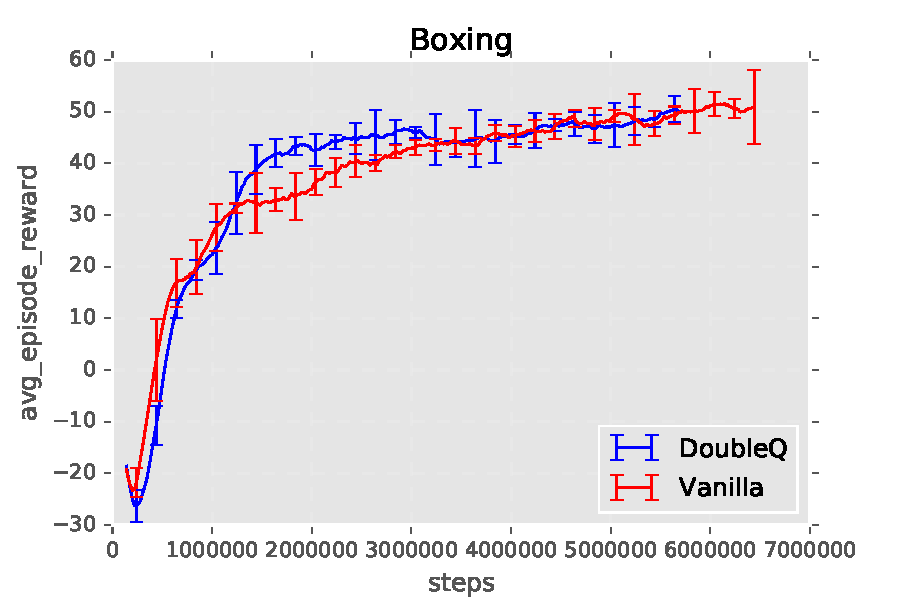
\includegraphics[width=0.5\textwidth]{../results/Boxing/Comparisons/DoubleQ/DoubleQ-baseline-avg_episode_reward.pdf}
    \label{boxing Double DQN}
    \caption{Average Episode reward with Double DQN for Boxing}
\end{figure}

\begin{figure}[h!]
    \centering
    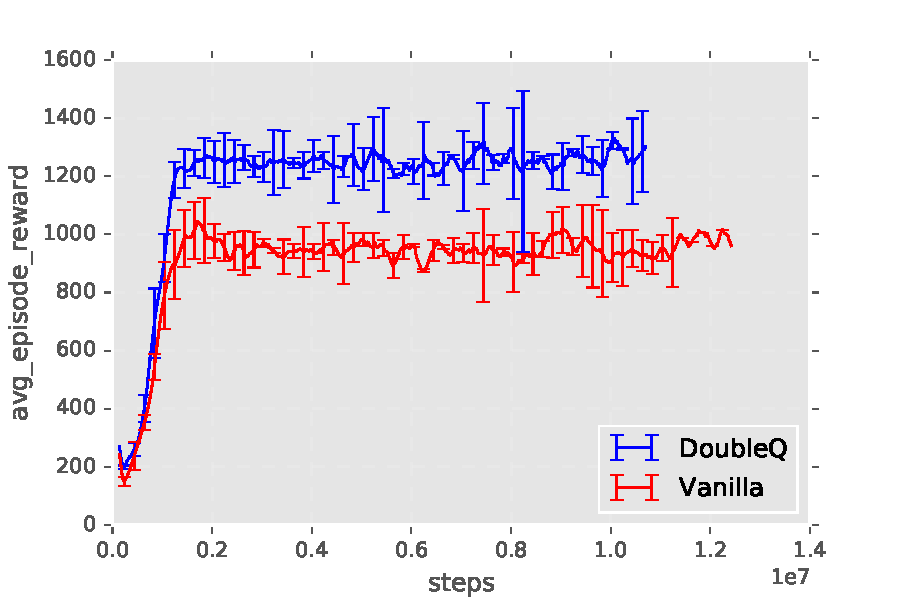
\includegraphics[width=0.5\textwidth]{../results/Krull/Comparisons/DoubleQ/DoubleQ-baseline-avg_episode_reward.pdf}
    \label{krull Double DQN}
    \caption{Average Episode reward with Double DQN for Krull}
\end{figure}

For the Atari Boxing game, it seems that the Double DQN tends to perform equally as the Vanilla DQN, but for Krull, we can clearly see that the average episode reward of double DQN lies higher than the baseline. Also do we see very clear the point, where decoupling of the selection and evaluation comes into its own. Both methods learn at an equal rate until a certain point, where Double DQN continues the slope of the learning rate and where the Vanilla DQN falls back in performance due it overoptimistic behaviour. The overoptimistic behaviour is visible in the average Q. We see that Vanilla DQN has a much higher Average Q value and Double DQN is able to estimate the Q value fairer. The distance between the two Average Q graphs, shows itself also in the graphs with the average episode rewards. For boxing is the distance rather small and do we see also a small distance between the average episode rewards, where this is the other way around for Krull.


\begin{figure}[h!]
    \centering
    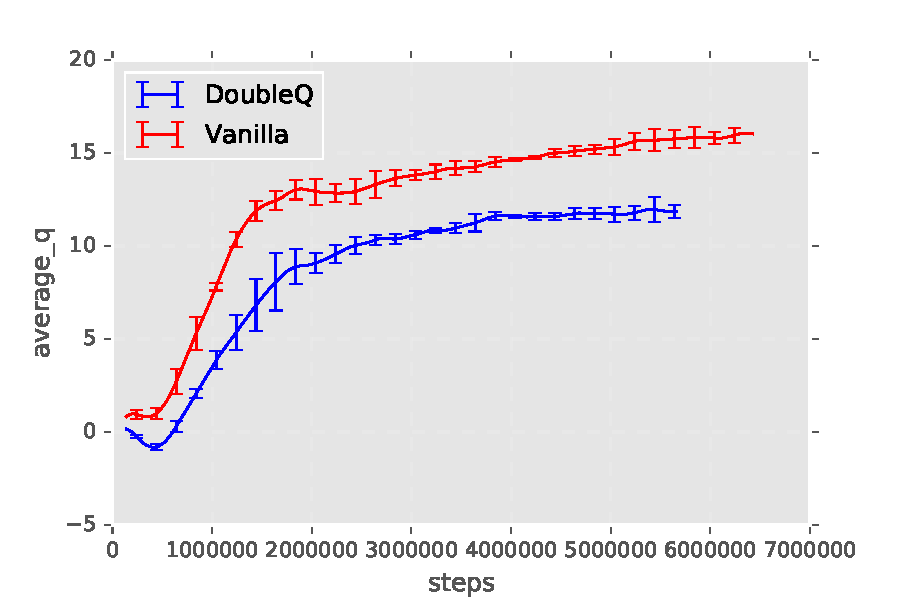
\includegraphics[width=0.5\textwidth]{../results/Boxing/Comparisons/DoubleQ/DoubleQ-baseline-average_q.pdf}
    \label{boxing Double DQN}
    \caption{Average Episode reward with Double DQN for Boxing}
\end{figure}

\begin{figure}[h!]
    \centering
    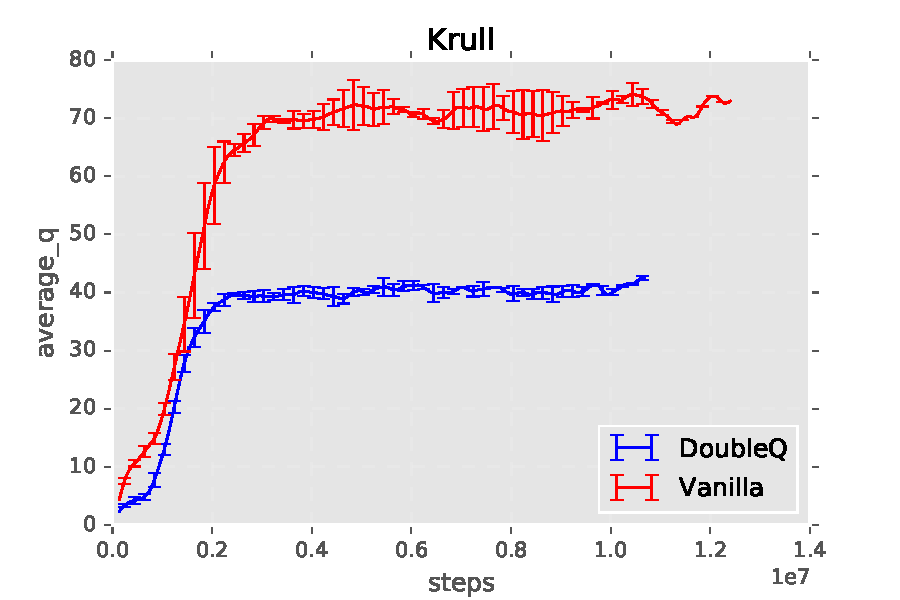
\includegraphics[width=0.5\textwidth]{../results/Krull/Comparisons/DoubleQ/DoubleQ-baseline-average_q.pdf}
    \label{krull Double DQN}
    \caption{Average Episode reward with Double DQN for Krull}
\end{figure}

All other results of this experiment can be found in appendix \ref{Appendix Double DQN}

\subsection{DQN with Prioritized Experience Replay}

Secondly, we ran the DQN with Priortized Experience Replay to learn to play the two games. We ran it with the defined hyper-parameters in \cite{schaul2015prioritized}: $\alpha=0.7$  and $\beta=0.3$

\begin{figure}[h!]
    \centering
    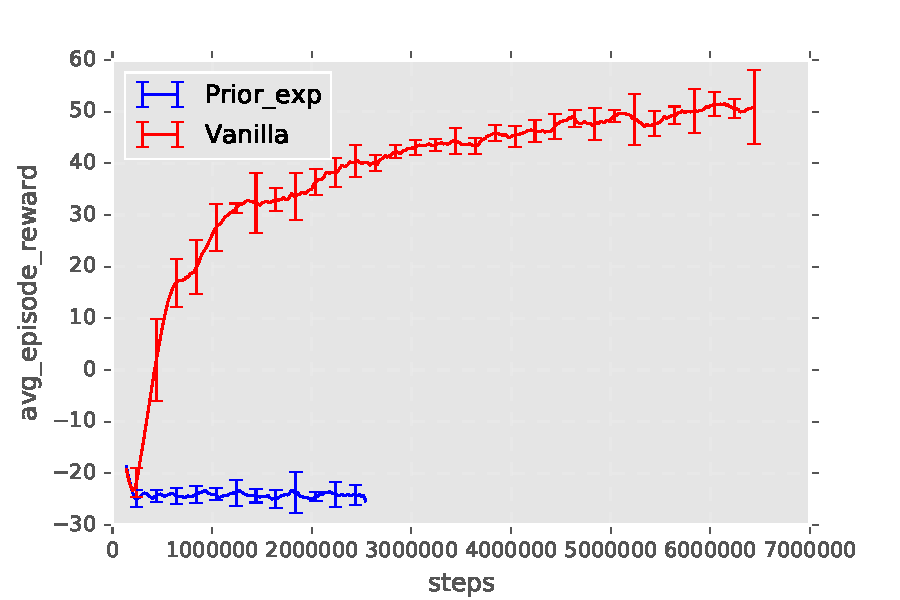
\includegraphics[width=0.5\textwidth]{../results/Boxing/Comparisons/Prior_exp/Prior_exp-baseline-avg_episode_reward.pdf}
    \label{boxing priorexp}
    \caption{Average Episode reward with Prioritized Experience Replay for Boxing}
\end{figure}

\begin{figure}[h!]
    \centering
    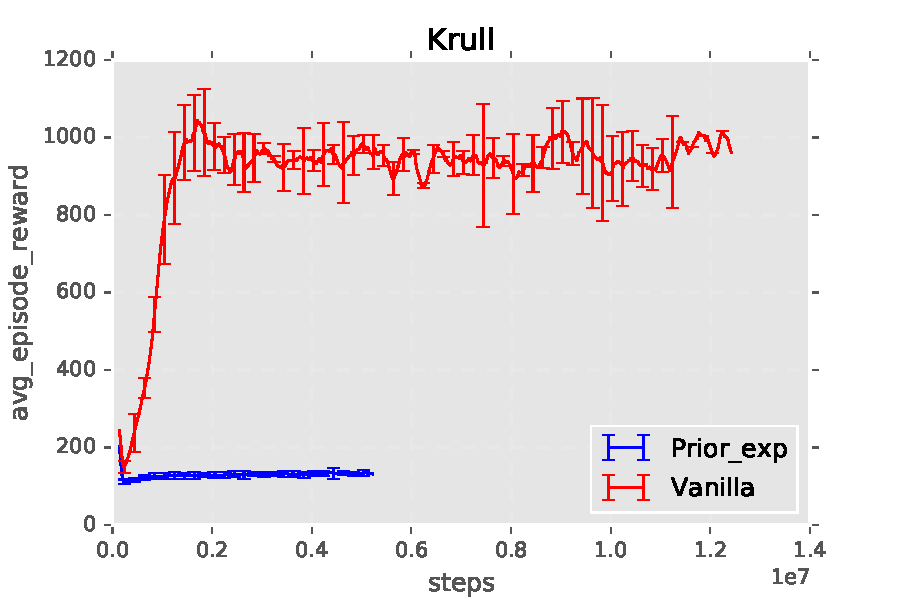
\includegraphics[width=0.5\textwidth]{../results/Krull/Comparisons/Prior_exp/Prior_exp-baseline-avg_episode_reward.pdf}
    \label{krull priorexp}
    \caption{Average Episode reward with Prioritized Experience Replay for Krull}
\end{figure}

As we can see in figure \ref{krull priorexp} and \ref{boxing priorexp}, is there a drastically difference with the results from Double DQN. It seems simple to learn nothing.Also the average Q shows dramatic bad results. In figure \ref{average q prior exp}, we see that the average q value of prior experience goes in the opposite direction, compared to the baseline. The bad results are not environment dependant, since we see the same bad results for both games.

\begin{figure}[h!]
    \centering
    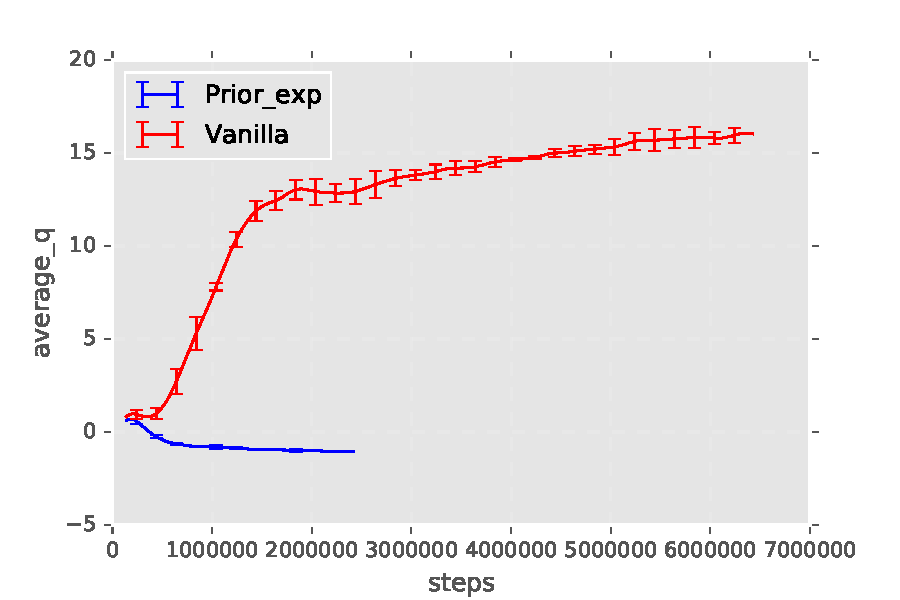
\includegraphics[width=0.5\textwidth]{../results/Boxing/Comparisons/Prior_exp/Prior_exp-baseline-average_q.pdf}
    \label{average q prior exp}
    \caption{Average Q with Prioritized Experience Repla yfor Boxing}
\end{figure}

\begin{figure}[h!]
    \centering
    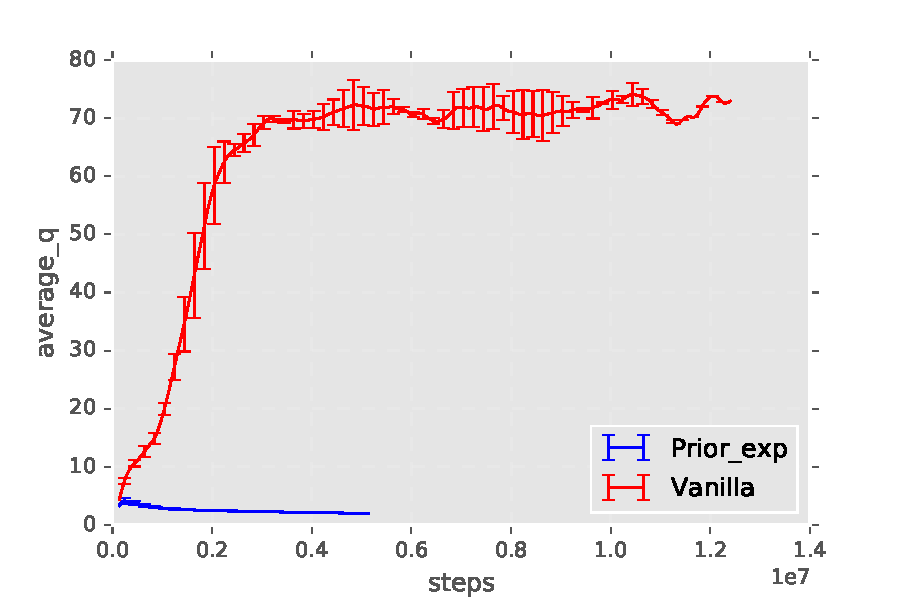
\includegraphics[width=0.5\textwidth]{../results/Krull/Comparisons/Prior_exp/Prior_exp-baseline-average_q.pdf}
    \caption{Average Episode reward with Prioritized Experience Replay for Krull}
\end{figure}

Our thoughts after seeing these results were a bug. We must have implemented something wrong. Although, after further research nothing seems really to be wrong. The Prioritized Experience Replay is in the same way implemented as the normal experience replay. The only difference is the implemented memory and how it selects is transitions. Our hypothesis of the bug was a bad selection distribution, which causes instability. Surprisingly, tests showed that the implemented distribution was just fine and behaves exactly as described. Figure \ref{hist} shows one of these results, where a histogram shows the requested indexes to the replay memory.


\begin{figure}[h!]
    \centering
    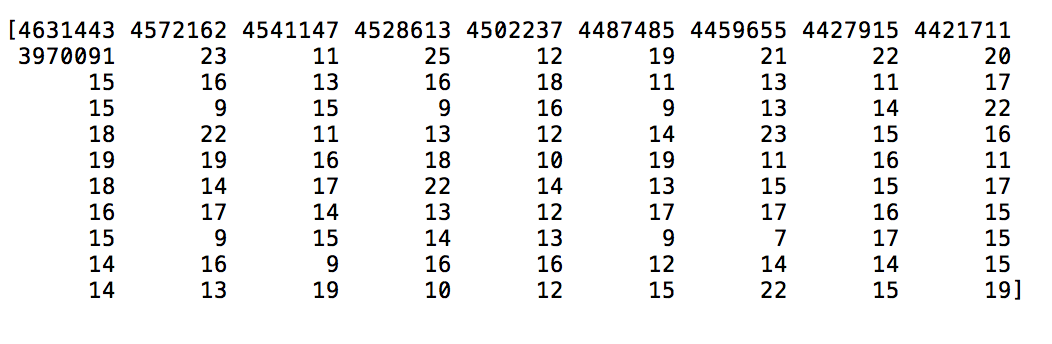
\includegraphics[width=0.5\textwidth]{../results/hist_100.png}
    \label{hist}
    \caption{A Histogram of 100 bins with all the requested ranks of the heap. As we can see are all the requested indexes mostly for the value who ranked the higestes in the heap. Exactly the behaviour we want too.}
\end{figure}

The complete results can be found in Appendix \ref{Appendix Priority Experience Replay}

\subsection{Implementation Details}

To speed up the working of Prioritized Experience Replay, we implemented a binary heap. This makes finding the maximum priority $O(1)$ and updating the priority values $O(log(n))$. The transitions get sorted in the binary heap based on their priority. The first transition in the heap gets initialised with one. When another transition is added to the memory is, it gets assigned the value of maximum priority currently in the heap, such that it will be replayed at least once. With an update, are the priorities of the replayed transitions incremented with the TD-error.


\subsection{Empirical Results of Prioritized Double DQN}

The last is experiment we conducted, is the combination of both adjustments, namely a Double DQN with Prioritized Experience Replay. 

\begin{figure}[h!]
    \centering
    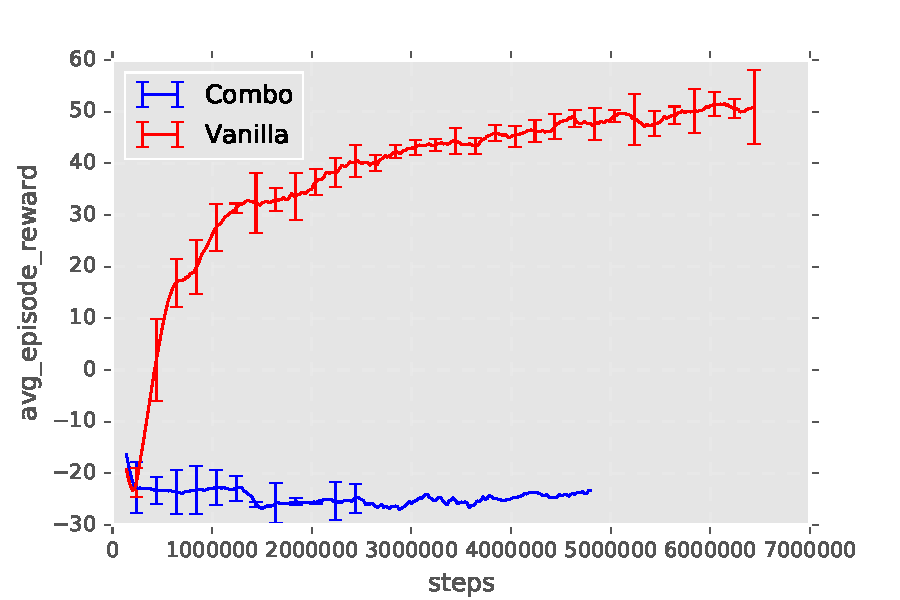
\includegraphics[width=0.5\textwidth]{../results/Boxing/Comparisons/Combo/Combo-baseline-avg_episode_reward.pdf}
    \label{boxing Double DQN}
    \caption{Average Episode reward with Double DQN and Prioritized Experience Replay for Boxing}
\end{figure}

\begin{figure}[h!]
    \centering
    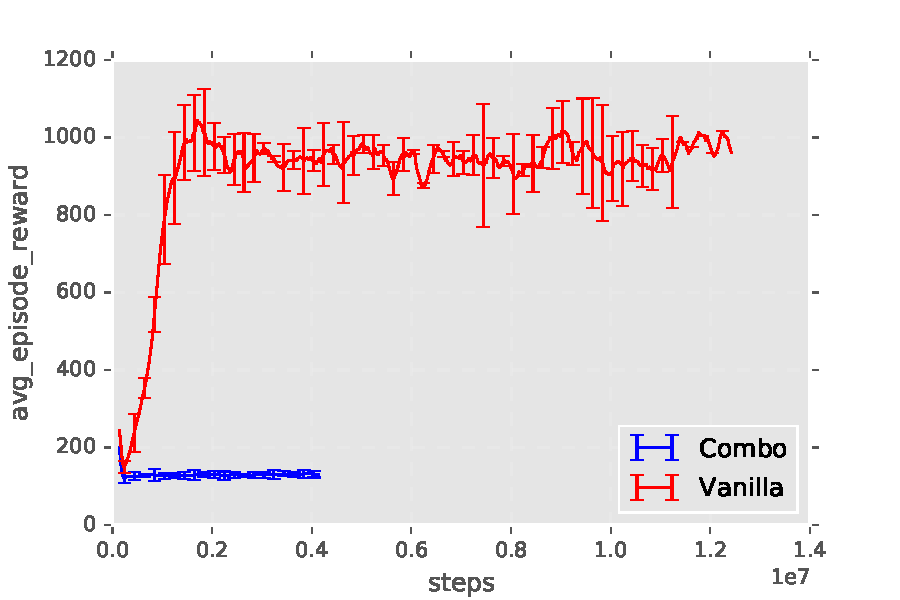
\includegraphics[width=0.5\textwidth]{../results/Krull/Comparisons/Combo/Combo-baseline-avg_episode_reward.pdf}
    \label{krull Double DQN}
    \caption{Average Episode reward with Double DQN and Prioritized Experience Replay for Krull}
\end{figure}


We see the same behaviour as with Priortized Experience Replay alone. The positive effect of Double DQN, seems not to have an impact on the terrible performance of the Prioritized experience replay. It shows exactly the same behaviour.

The complete results can be found in appendix \ref{Appendix Priority Experience Replay Double DQN}

\subsection{Side Note}
It was a real struggle to realise all the experiments.
We know that the experimental setup is not ideal. 5 runs for each experiment and a low amount of total steps makes the results less accurate. The reason is the limited time frame, which caused a lot of trouble. The initial idea was to conduct the experiments with the hyper-parameters of the original paper by \cite{mnih2015human}. Soon it became clear that an experiment with a memory-size of 1 million and 50 million steps, would not finish in time. As suggested, we tried to reduce the frame size to 42x42, but this resulted in almost no learning for several Atari games. Eventually after a lot of side-experiments, we ended up with the configuration suggested in \ref{Hyper parameters} and the two Atari games Krull and Boxing. Both of these games are selected based on their fast learning rate and good performance in a limited configuration. The limited time frame for this project had also an impact on the amount of runs. Ideally we liked to conduct 10 runs or more for each experiment. This meant that we had to run 80 runs at the same time on the hydracluster. Unfortunately, this seemed to be not possible, because or the UserRAMLimit. Also balancing the runs and only assign 16gb to experiments that needed it, did not help. This resulted in several runs getting randomly killed after a few days. Eventually we succeed to create a stable experimental environment by doing only 5 runs per experiment. 

\section{Discussion}

Overall we can say that we are not completely satisfied with our results. Especially, the bad results of Prioritized Experience Replay disappoints us. Extensive research towards the behaviour of our implementation shows that it works as described in the original paper. This led to a big frustration. Especially since it is shown by \cite{schaul2015prioritized} to be possible to achieve better results. Of course do we also need to nuance our results, since we have evaluated them over a limited stepsize. Although, that the two games were specifically chosen because of their fast learning rate and significant improvement with these two techniques. To conclude we say that we implemented a prioritized experience replay that needs to be improved and at last we also successfully implemented and Double DQN network, which showed successful results. 

% The following two commands are all you need in the
% initial runs of your .tex file to
% produce the bibliography for the citations in your paper.
\bibliographystyle{apalike}
\bibliography{bib}  % sigproc.bib is the name of the Bibliography in this case
% You must have a proper ".bib" file
%  and remember to run:
% latex bibtex latex latex
% to resolve all references
%{}
% ACM needs 'a single self-contained file'!

\appendix
\section{Double DQN}\label{Appendix Double DQN}

\subsection{Krull}\label{Appendix krull}

\begin{figure}[h!]
    \centering
    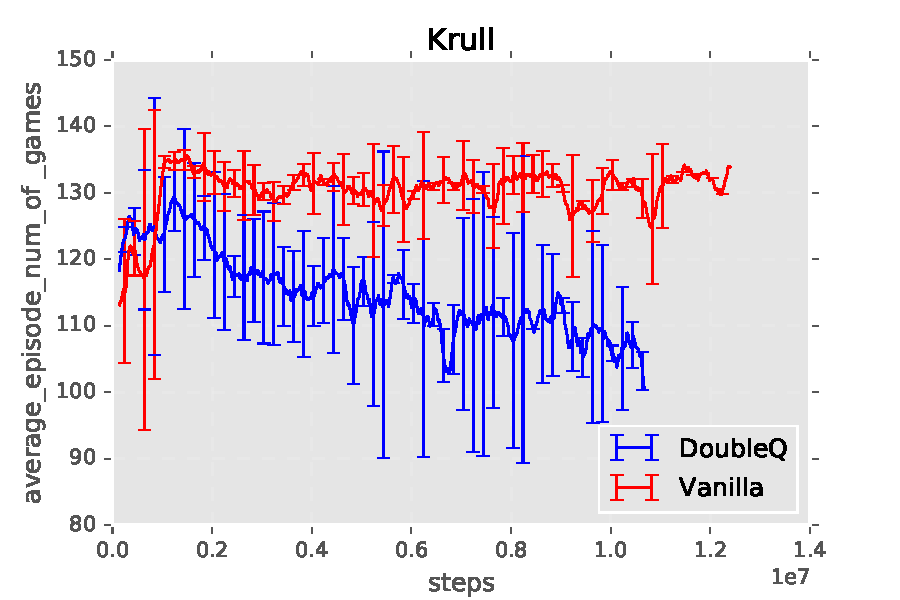
\includegraphics[width=0.5\textwidth]{../results/Krull/Comparisons/DoubleQ/DoubleQ-baseline-average_episode_num_of_games.pdf}
\end{figure}


\begin{figure}
    \centering
    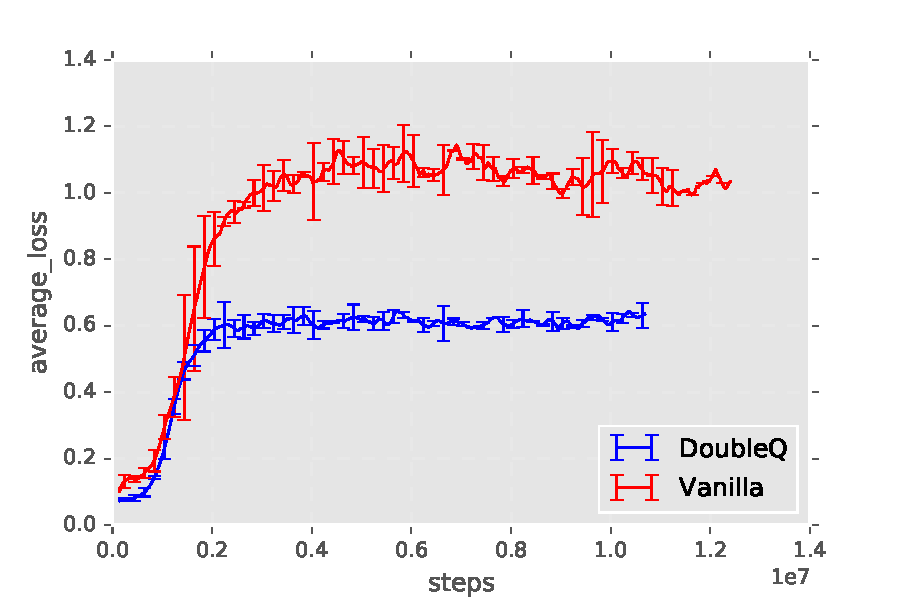
\includegraphics[width=0.5\textwidth]{../results/Krull/Comparisons/DoubleQ/DoubleQ-baseline-average_loss.pdf}
\end{figure}


\begin{figure}[h!]
    \centering
    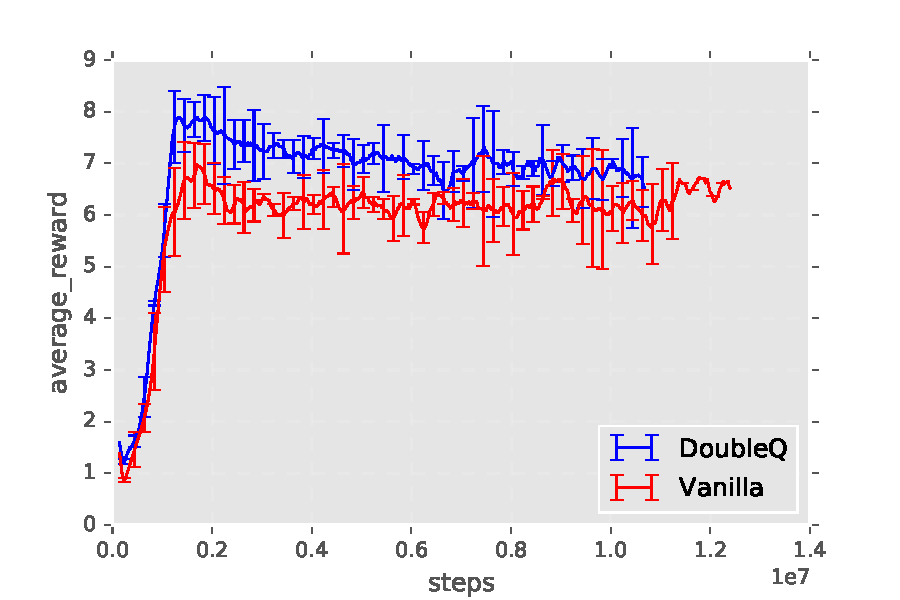
\includegraphics[width=0.5\textwidth]{../results/Krull/Comparisons/DoubleQ/DoubleQ-baseline-average_reward.pdf}
\end{figure}

\begin{figure}[h!]
    \centering
    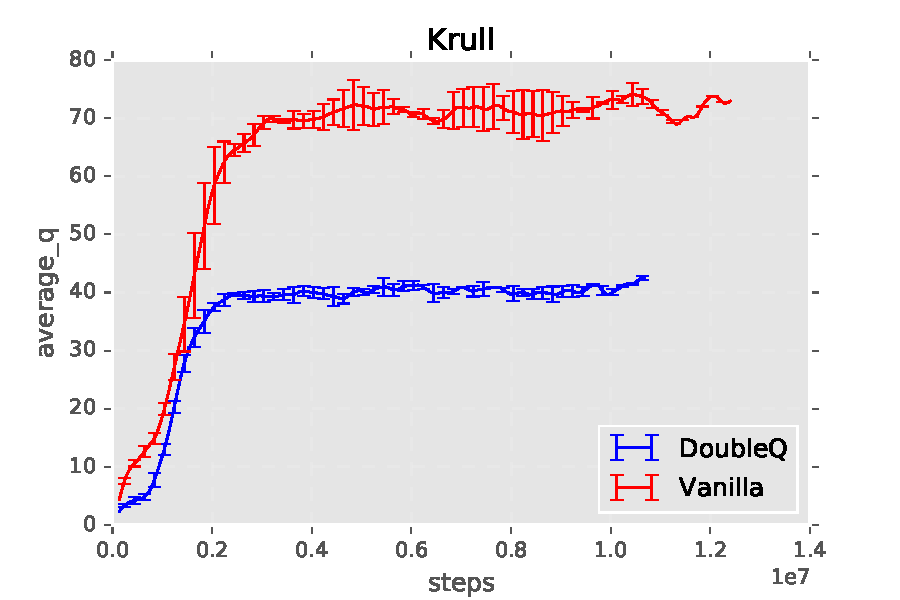
\includegraphics[width=0.5\textwidth]{../results/Krull/Comparisons/DoubleQ/DoubleQ-baseline-average_q.pdf}
\end{figure}

\begin{figure}[h!]
    \centering
    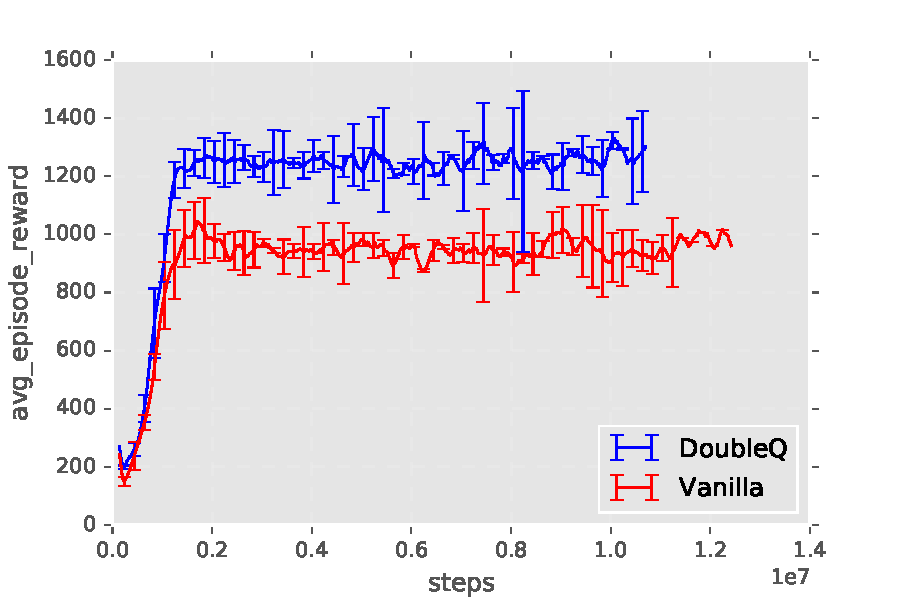
\includegraphics[width=0.5\textwidth]{../results/Krull/Comparisons/DoubleQ/DoubleQ-baseline-avg_episode_reward.pdf}
\end{figure}

\begin{figure}[h!]
    \centering
    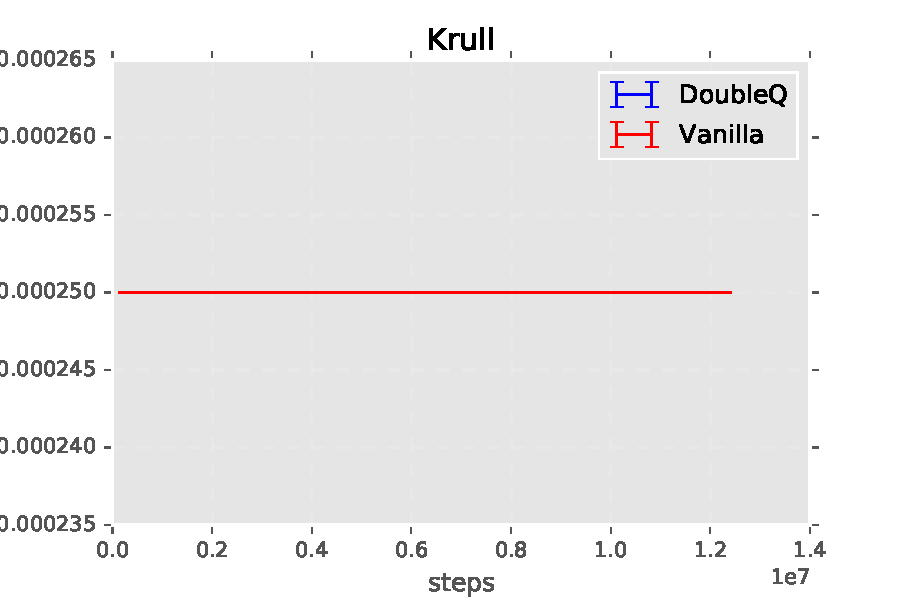
\includegraphics[width=0.5\textwidth]{../results/Krull/Comparisons/DoubleQ/DoubleQ-baseline-learning_rate.pdf}
\end{figure}


\begin{figure}[h!]
    \centering
    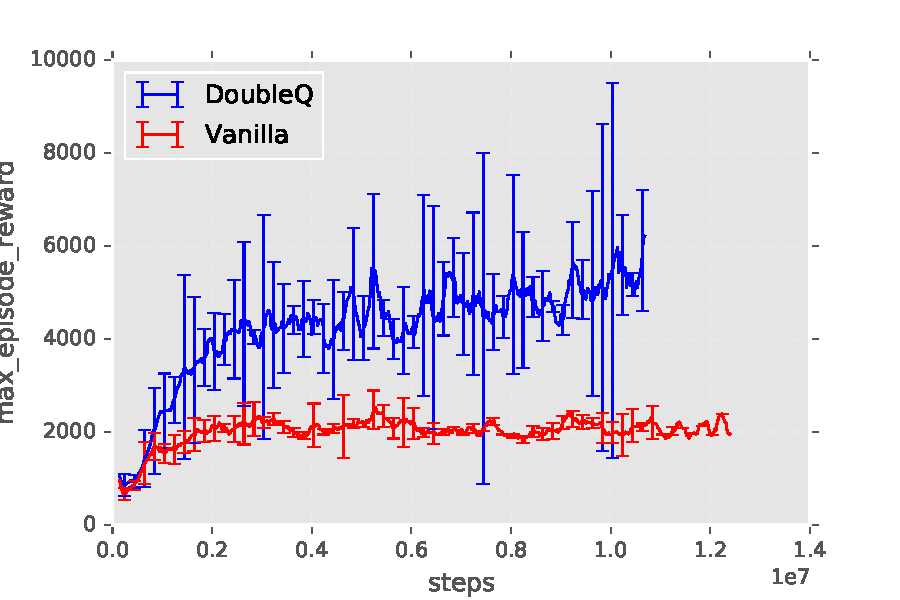
\includegraphics[width=0.5\textwidth]{../results/Krull/Comparisons/DoubleQ/DoubleQ-baseline-max_episode_reward.pdf}
\end{figure}


\begin{figure}[h!]
    \centering
    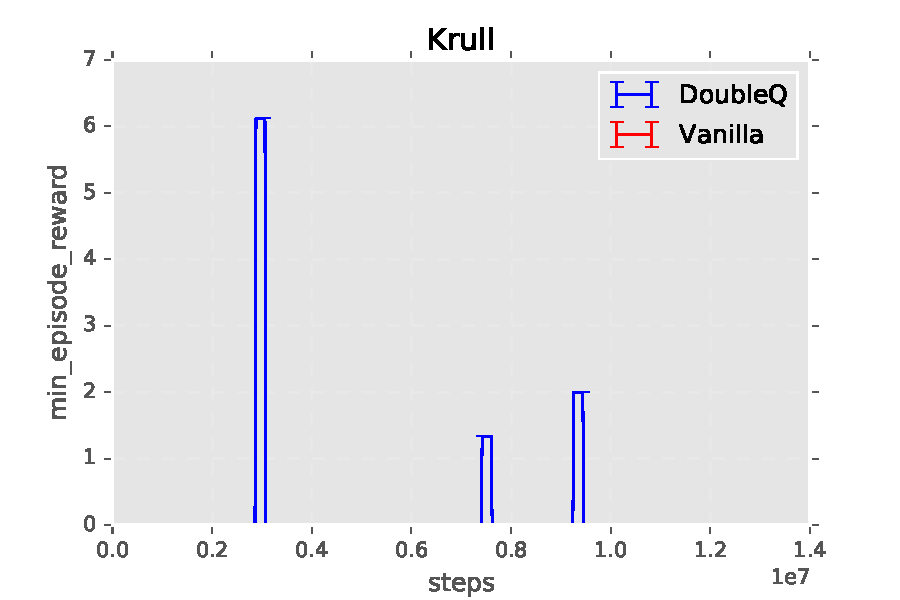
\includegraphics[width=0.5\textwidth]{../results/Krull/Comparisons/DoubleQ/DoubleQ-baseline-min_episode_reward.pdf}
\end{figure}

\FloatBarrier
\subsection{Boxing}\label{Appendix boxing double}

\begin{figure}[h!]
    \centering
    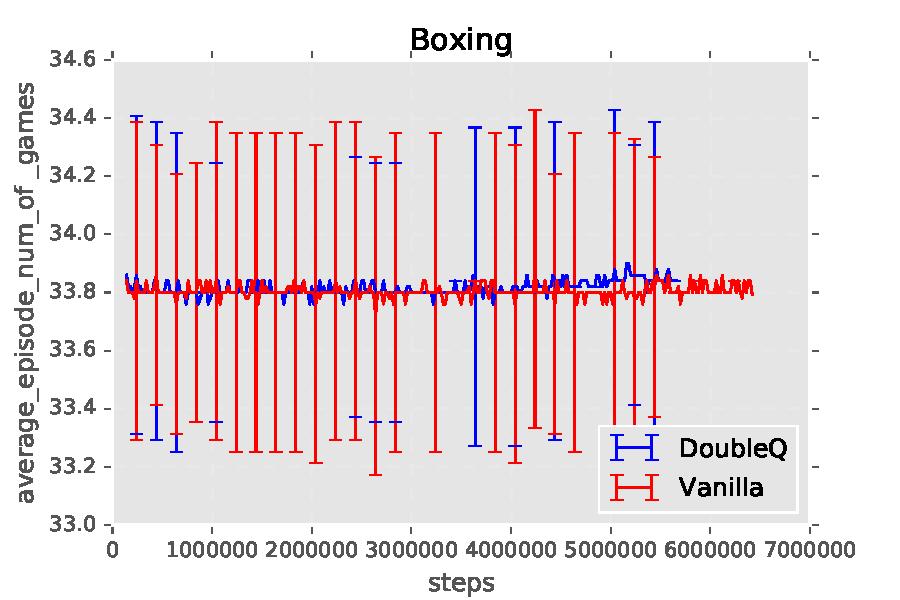
\includegraphics[width=0.5\textwidth]{../results/Boxing/Comparisons/DoubleQ/DoubleQ-baseline-average_episode_num_of_games.pdf}
\end{figure}


\begin{figure}[h!]
    \centering
    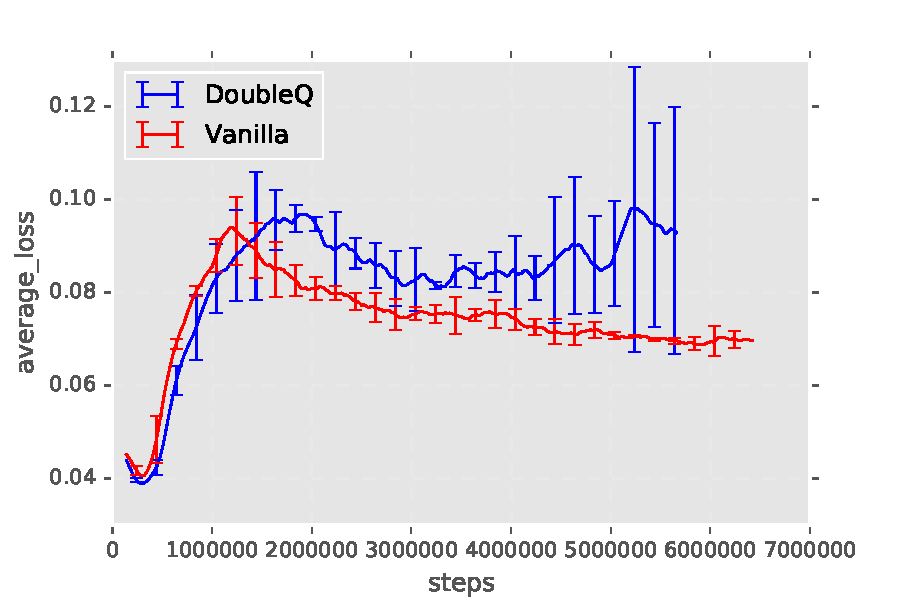
\includegraphics[width=0.5\textwidth]{../results/Boxing/Comparisons/DoubleQ/DoubleQ-baseline-average_loss.pdf}
\end{figure}


\begin{figure}[h!]
    \centering
    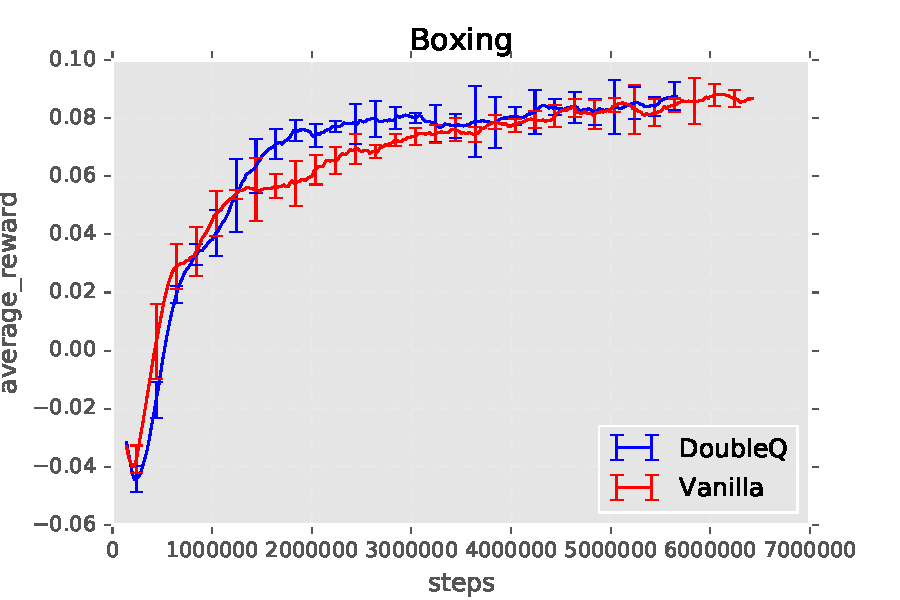
\includegraphics[width=0.5\textwidth]{../results/Boxing/Comparisons/DoubleQ/DoubleQ-baseline-average_reward.pdf}
\end{figure}

\begin{figure}[h!]
    \centering
    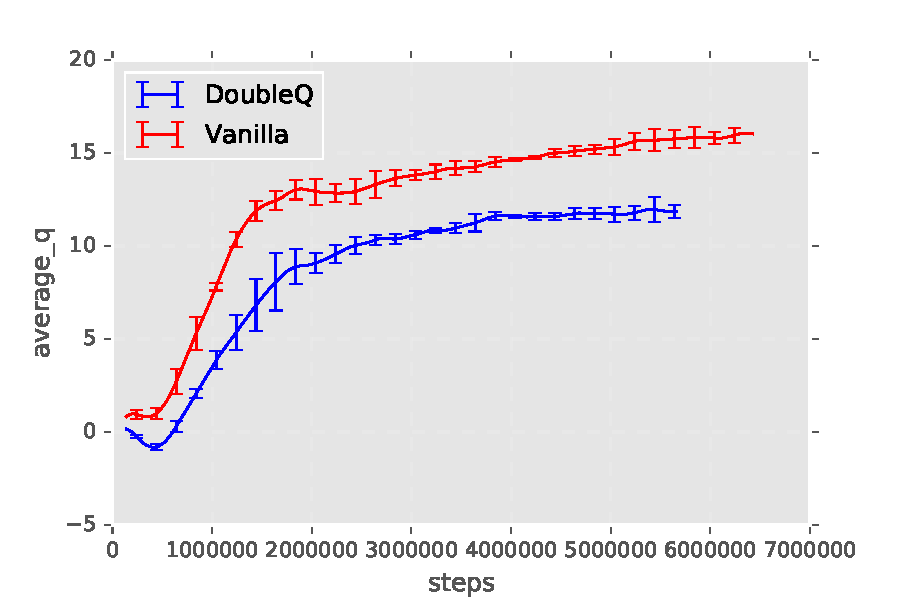
\includegraphics[width=0.5\textwidth]{../results/Boxing/Comparisons/DoubleQ/DoubleQ-baseline-average_q.pdf}
\end{figure}

\begin{figure}[h!]
    \centering
    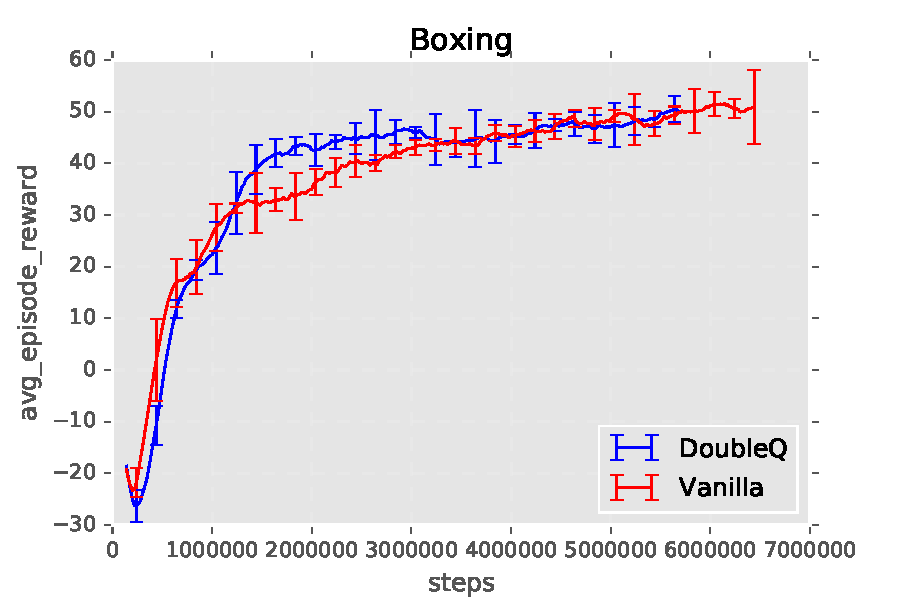
\includegraphics[width=0.5\textwidth]{../results/Boxing/Comparisons/DoubleQ/DoubleQ-baseline-avg_episode_reward.pdf}
\end{figure}

\begin{figure}[h!]
    \centering
    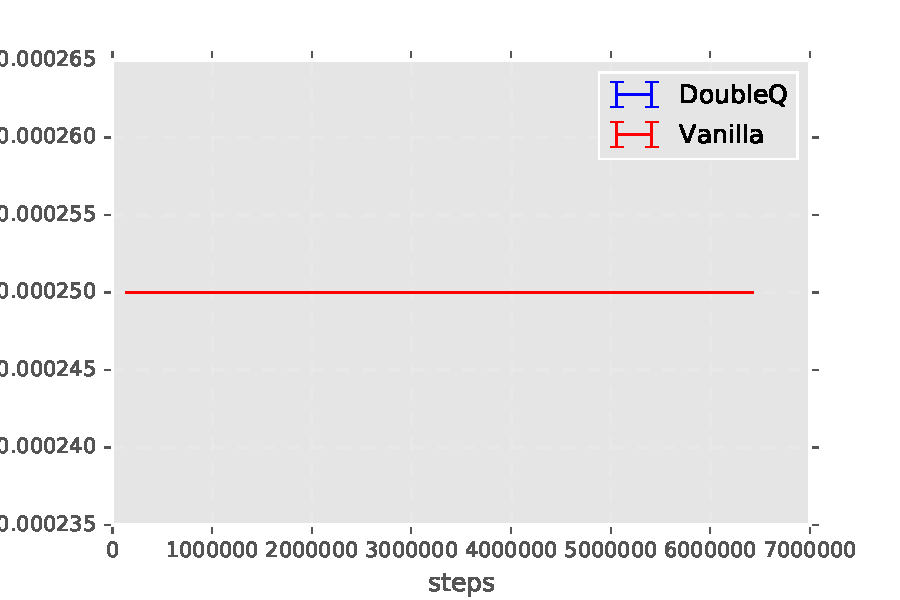
\includegraphics[width=0.5\textwidth]{../results/Boxing/Comparisons/DoubleQ/DoubleQ-baseline-learning_rate.pdf}
\end{figure}


\begin{figure}[h!]
    \centering
    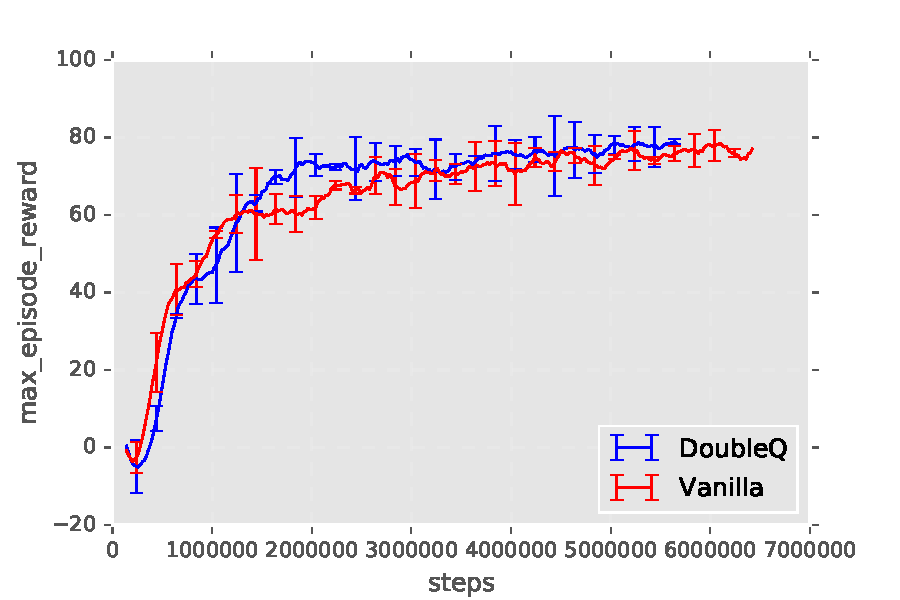
\includegraphics[width=0.5\textwidth]{../results/Boxing/Comparisons/DoubleQ/DoubleQ-baseline-max_episode_reward.pdf}
\end{figure}


\begin{figure}[h!]
    \centering
    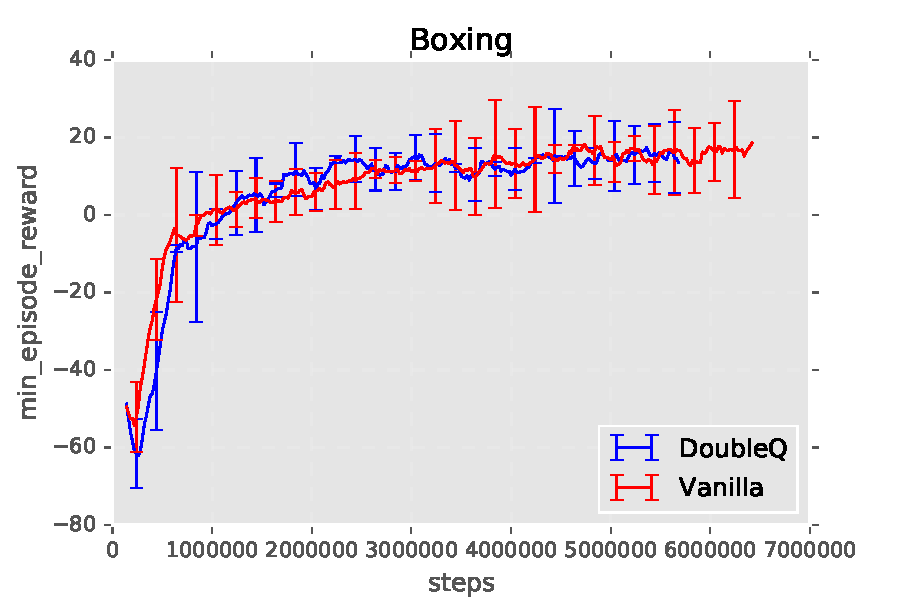
\includegraphics[width=0.5\textwidth]{../results/Boxing/Comparisons/DoubleQ/DoubleQ-baseline-min_episode_reward.pdf}
\end{figure}
\FloatBarrier


\section{Priority Experience Replay}\label{Appendix Priority Experience Replay}

\subsection{Krull}\label{Appendix prior krill}

\begin{figure}
    \centering
    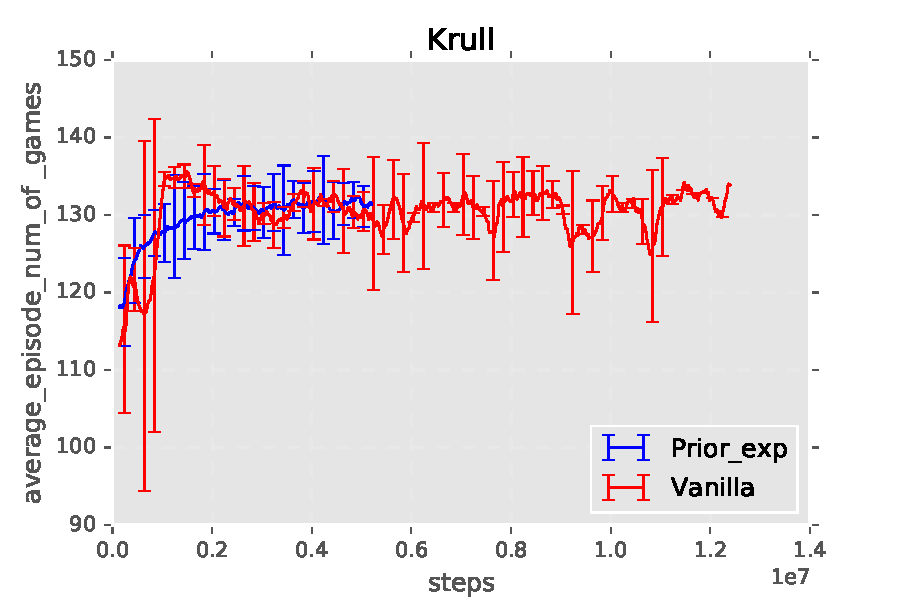
\includegraphics[width=0.5\textwidth]{../results/Krull/Comparisons/Prior_exp/Prior_exp-baseline-average_episode_num_of_games.pdf}
\end{figure}

\begin{figure}
    \centering
    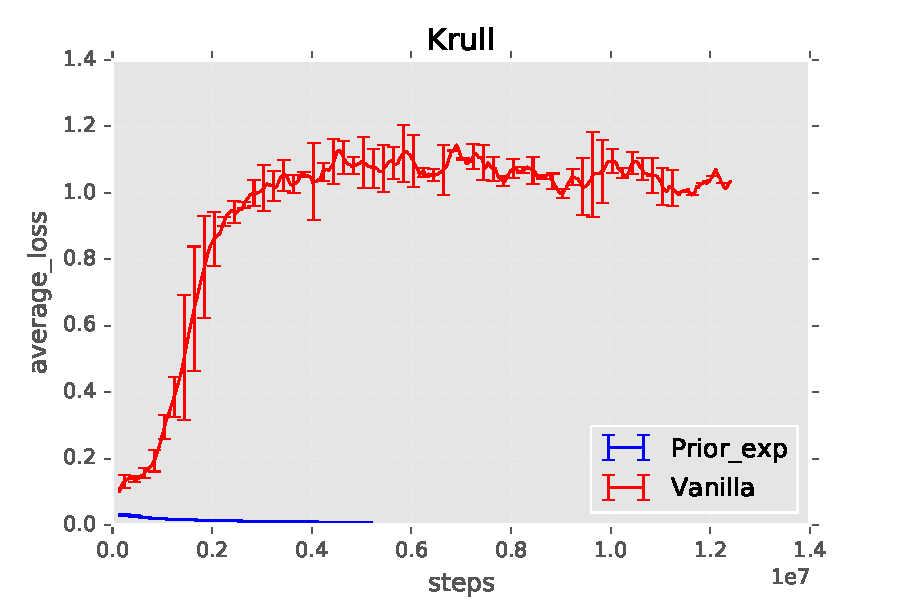
\includegraphics[width=0.5\textwidth]{../results/Krull/Comparisons/Prior_exp/Prior_exp-baseline-average_loss.pdf}
\end{figure}


\begin{figure}
    \centering
    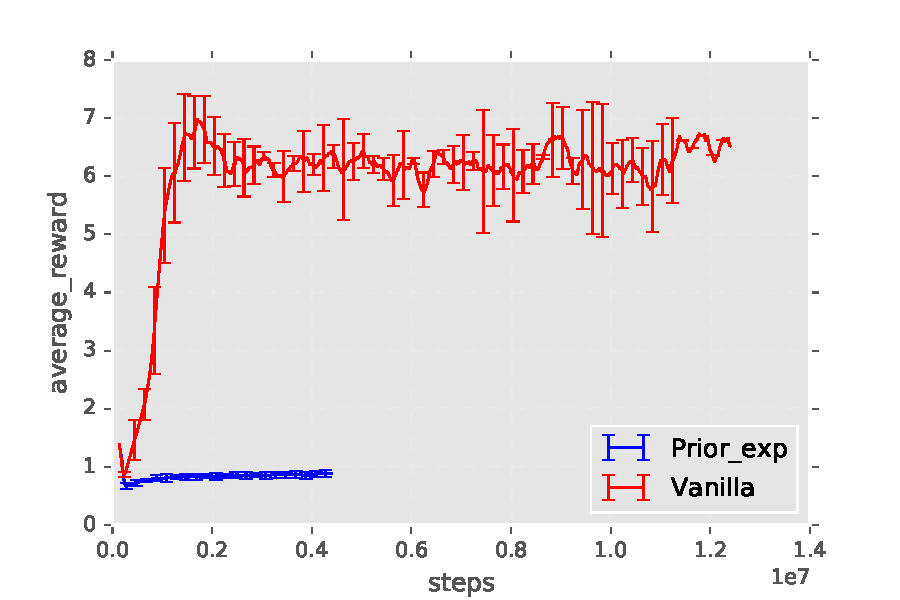
\includegraphics[width=0.5\textwidth]{../results/Krull/Comparisons/Prior_exp/Prior_exp-baseline-average_reward.pdf}
\end{figure}

\begin{figure}
    \centering
    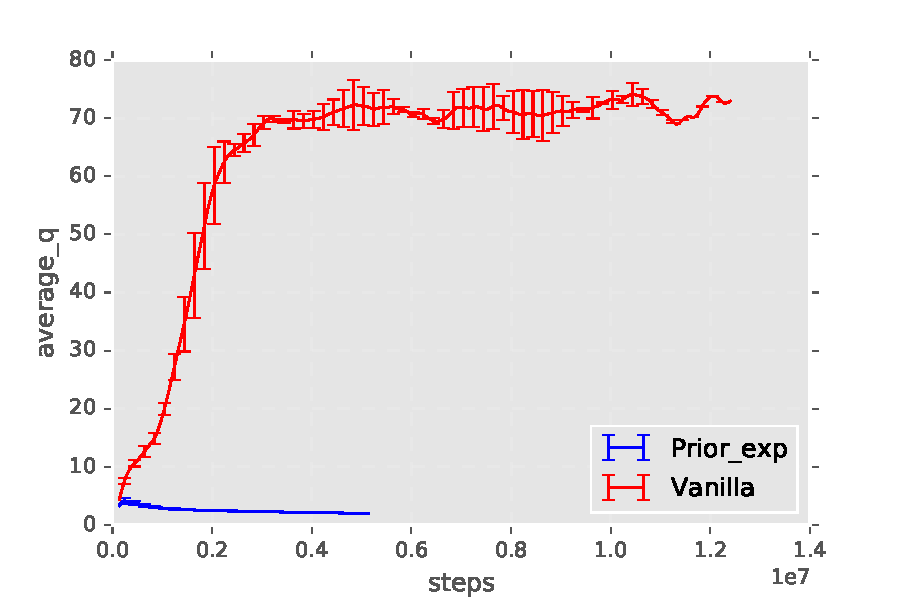
\includegraphics[width=0.5\textwidth]{../results/Krull/Comparisons/Prior_exp/Prior_exp-baseline-average_q.pdf}
\end{figure}

\begin{figure}
    \centering
    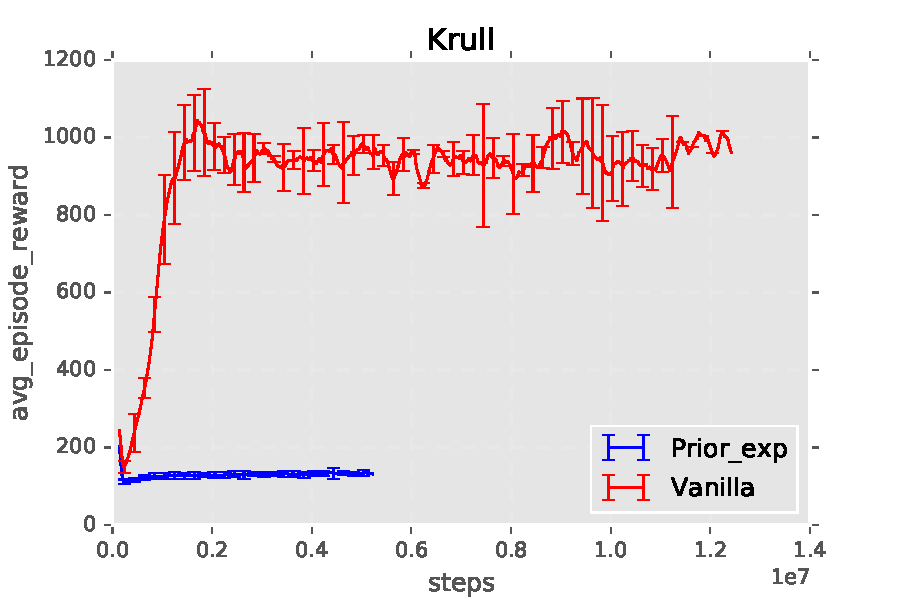
\includegraphics[width=0.5\textwidth]{../results/Krull/Comparisons/Prior_exp/Prior_exp-baseline-avg_episode_reward.pdf}
\end{figure}

\begin{figure}
    \centering
    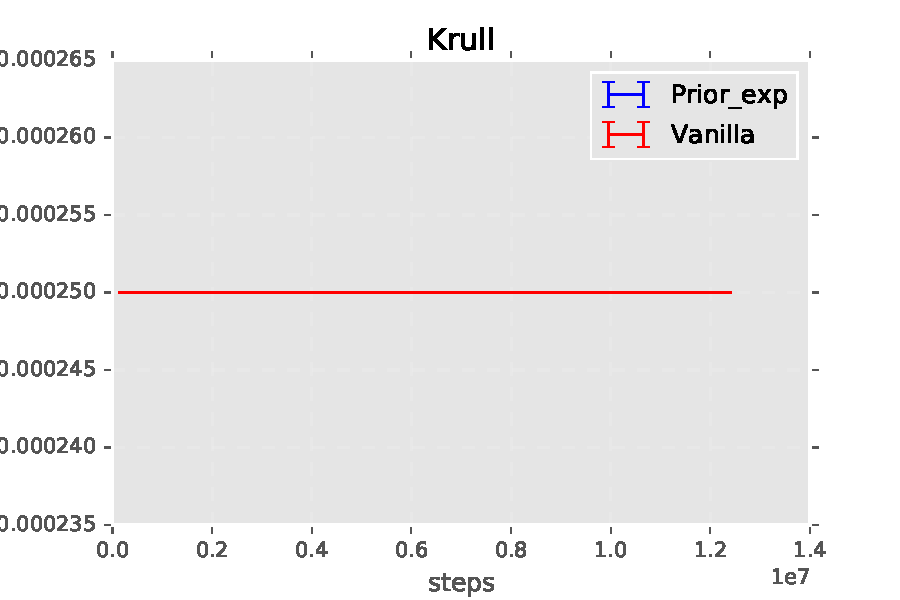
\includegraphics[width=0.5\textwidth]{../results/Krull/Comparisons/Prior_exp/Prior_exp-baseline-learning_rate.pdf}
\end{figure}


\begin{figure}
    \centering
    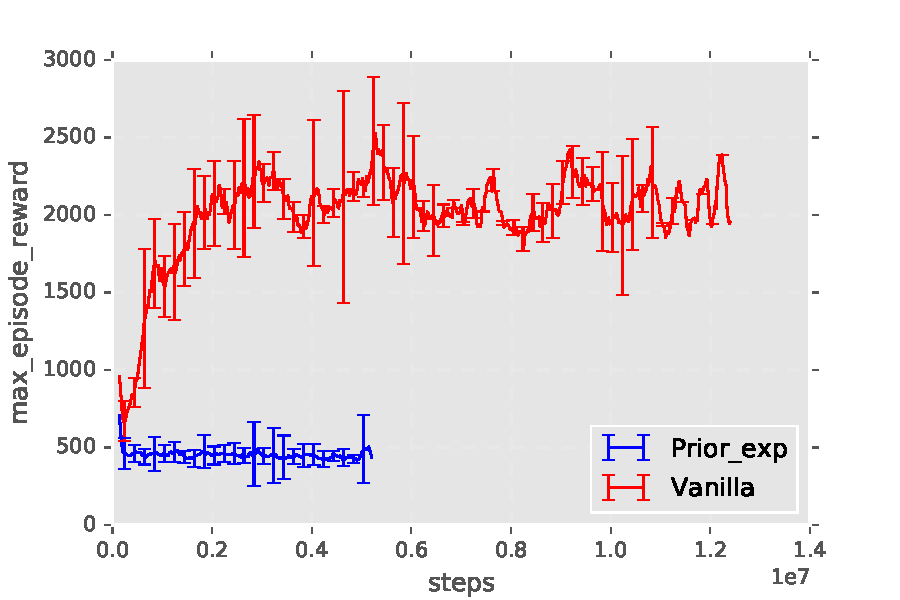
\includegraphics[width=0.5\textwidth]{../results/Krull/Comparisons/Prior_exp/Prior_exp-baseline-max_episode_reward.pdf}
\end{figure}


\begin{figure}
    \centering
    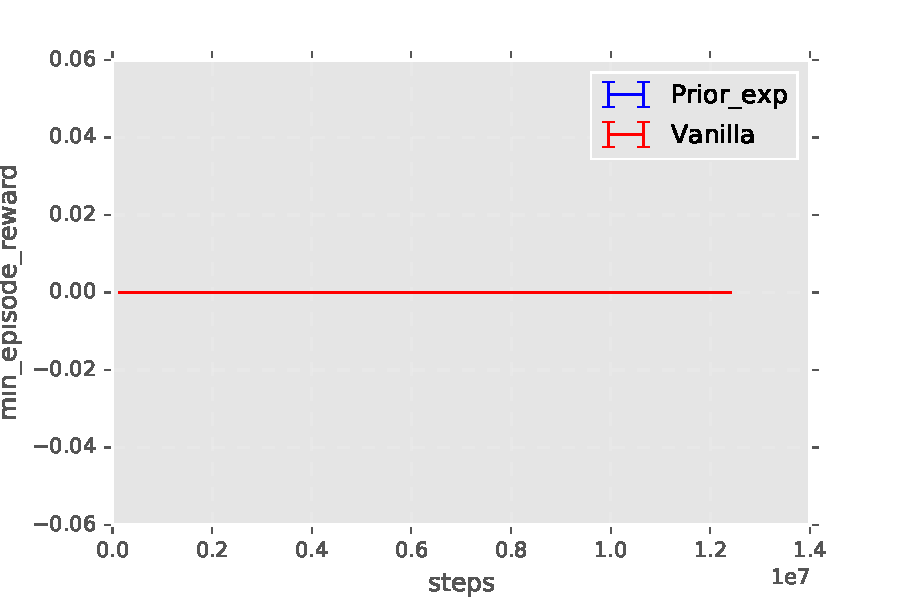
\includegraphics[width=0.5\textwidth]{../results/Krull/Comparisons/Prior_exp/Prior_exp-baseline-min_episode_reward.pdf}
\end{figure}
\FloatBarrier

\subsection{Boxing}\label{Appendix boxing prior}

\begin{figure}
    \centering
    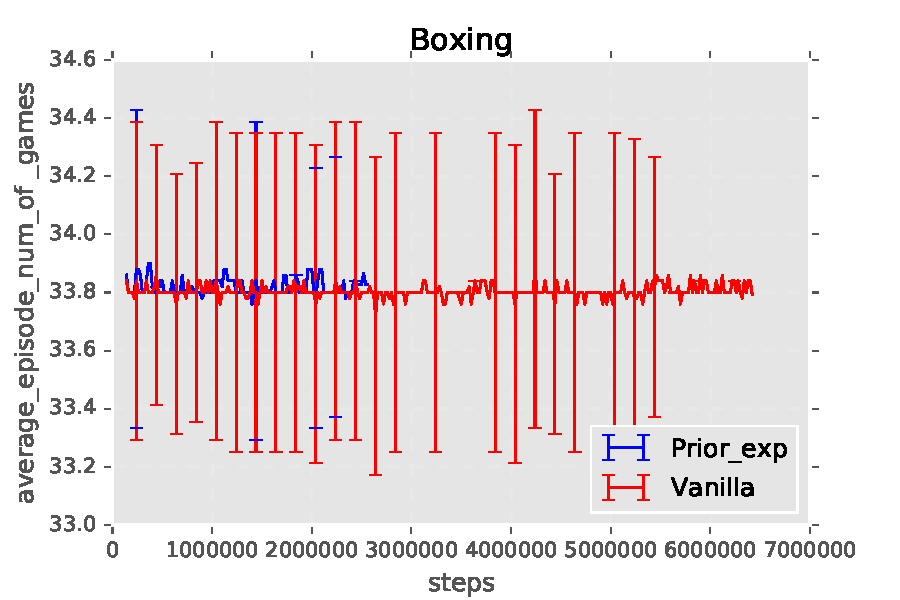
\includegraphics[width=0.5\textwidth]{../results/Boxing/Comparisons/Prior_exp/Prior_exp-baseline-average_episode_num_of_games.pdf}
\end{figure}


\begin{figure}
    \centering
    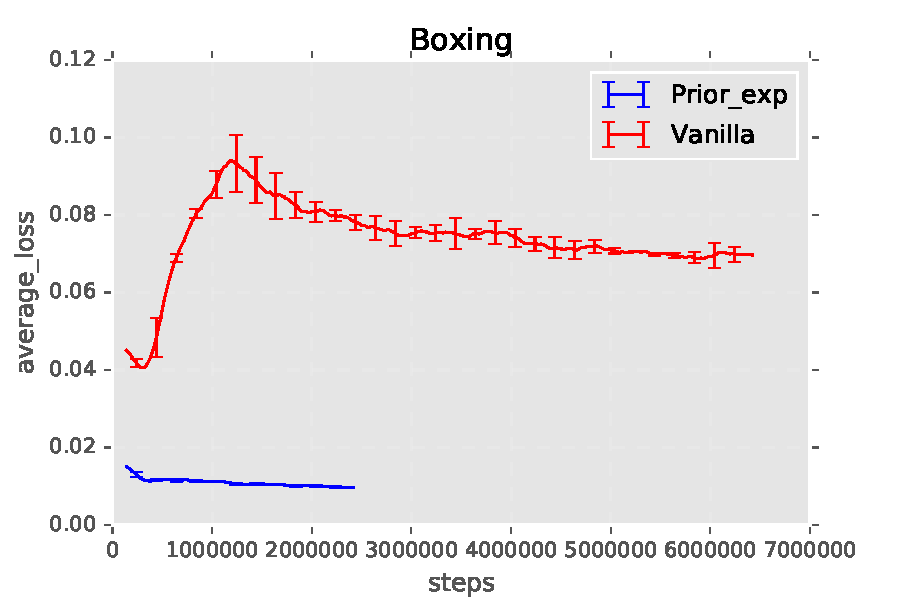
\includegraphics[width=0.5\textwidth]{../results/Boxing/Comparisons/Prior_exp/Prior_exp-baseline-average_loss.pdf}
\end{figure}


\begin{figure}
    \centering
    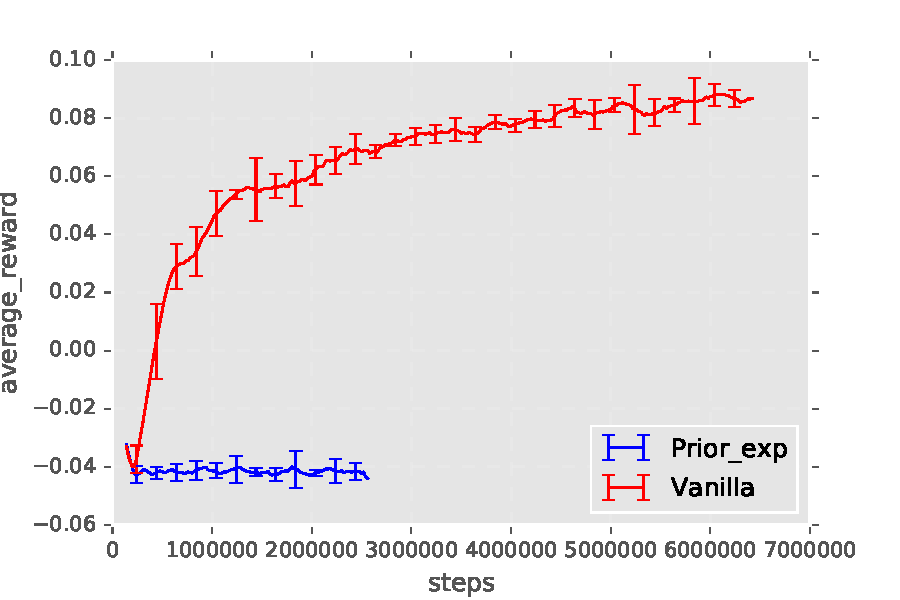
\includegraphics[width=0.5\textwidth]{../results/Boxing/Comparisons/Prior_exp/Prior_exp-baseline-average_reward.pdf}
\end{figure}

\begin{figure}
    \centering
    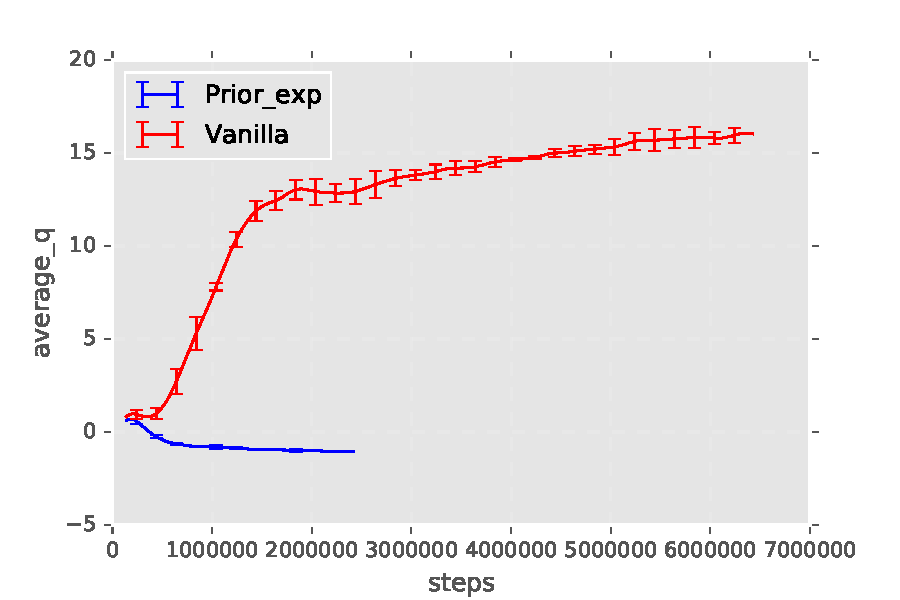
\includegraphics[width=0.5\textwidth]{../results/Boxing/Comparisons/Prior_exp/Prior_exp-baseline-average_q.pdf}
\end{figure}

\begin{figure}
    \centering
    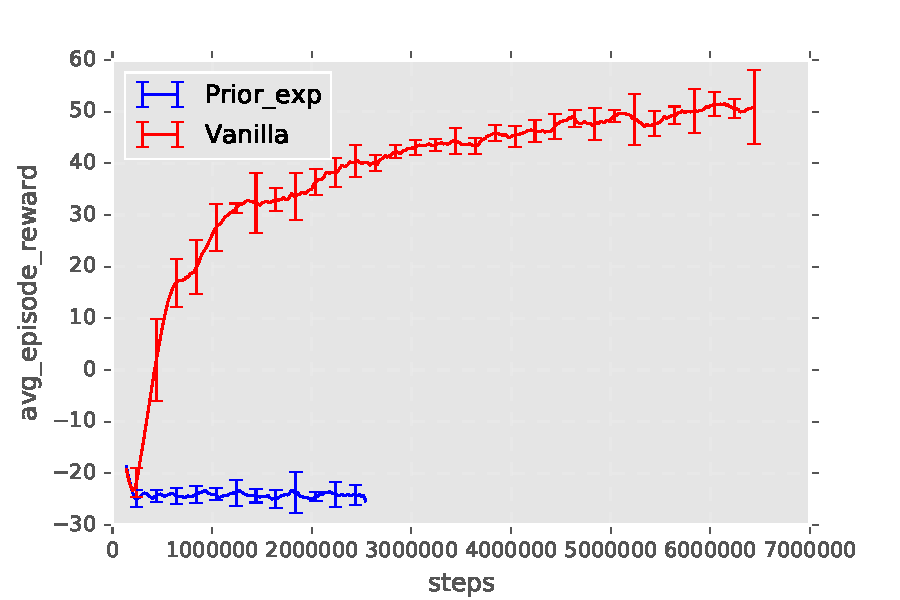
\includegraphics[width=0.5\textwidth]{../results/Boxing/Comparisons/Prior_exp/Prior_exp-baseline-avg_episode_reward.pdf}
\end{figure}

\begin{figure}
    \centering
    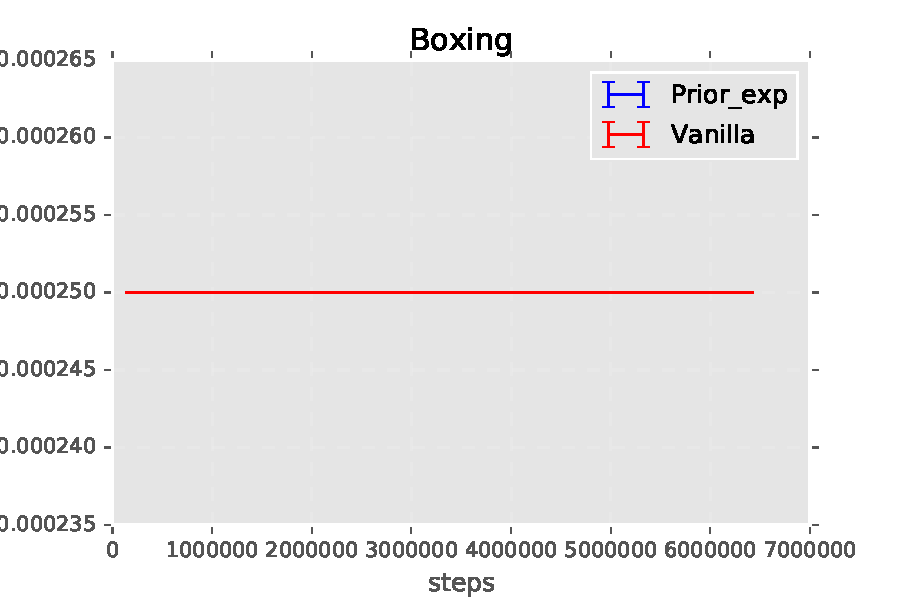
\includegraphics[width=0.5\textwidth]{../results/Boxing/Comparisons/Prior_exp/Prior_exp-baseline-learning_rate.pdf}
\end{figure}


\begin{figure}
    \centering
    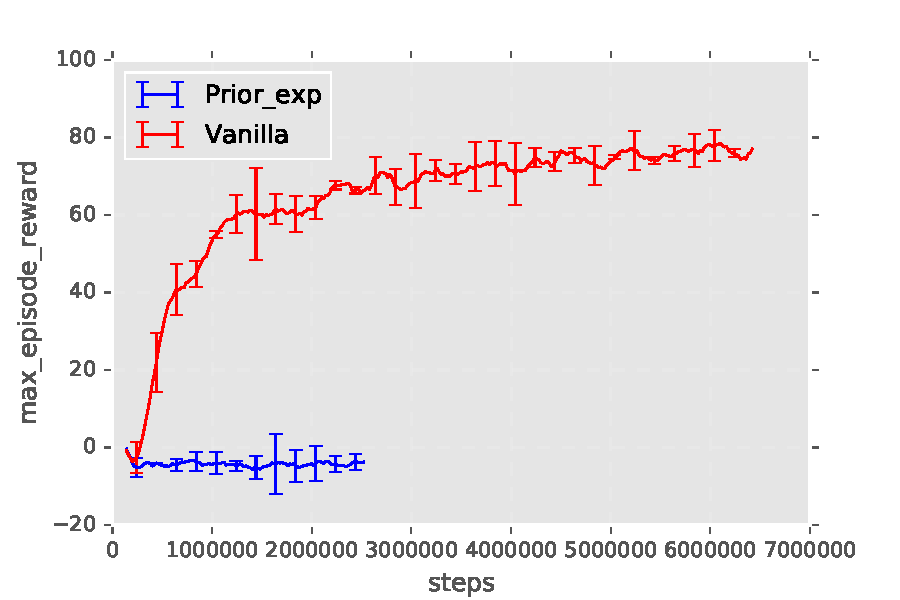
\includegraphics[width=0.5\textwidth]{../results/Boxing/Comparisons/Prior_exp/Prior_exp-baseline-max_episode_reward.pdf}
\end{figure}


\begin{figure}
    \centering
    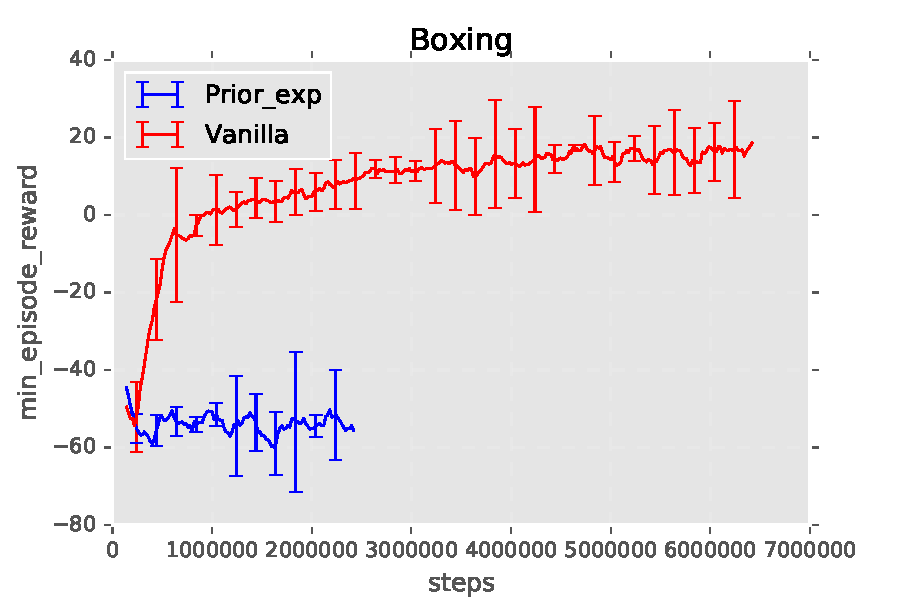
\includegraphics[width=0.5\textwidth]{../results/Boxing/Comparisons/Prior_exp/Prior_exp-baseline-min_episode_reward.pdf}
\end{figure}

\FloatBarrier

\section{Priority Experience Replay wiht Double DQN}\label{Appendix Priority Experience Replay Double DQN}

\subsection{Krull}\label{Appendix prior krill}

\begin{figure}
    \centering
    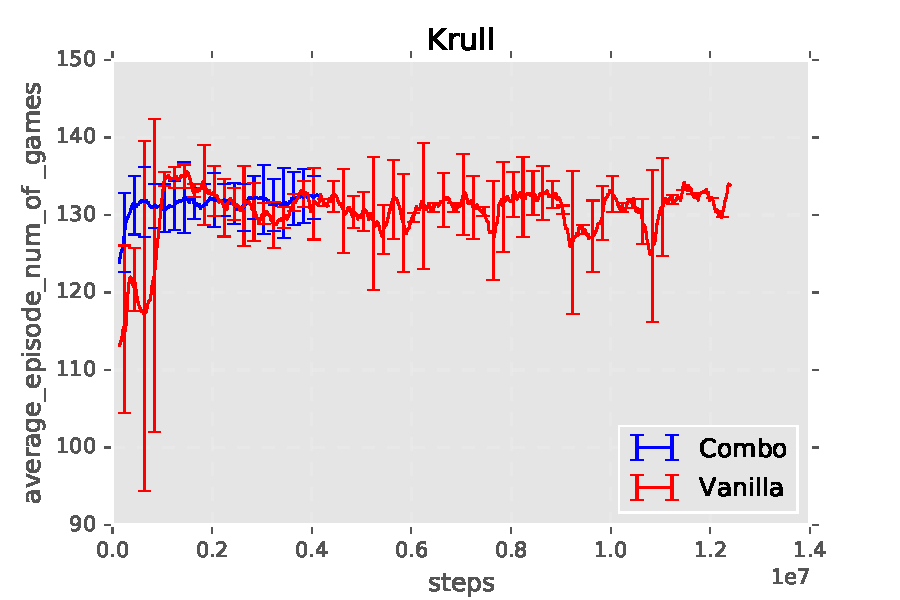
\includegraphics[width=0.5\textwidth]{../results/Krull/Comparisons/Combo/Combo-baseline-average_episode_num_of_games.pdf}
\end{figure}

\begin{figure}
    \centering
    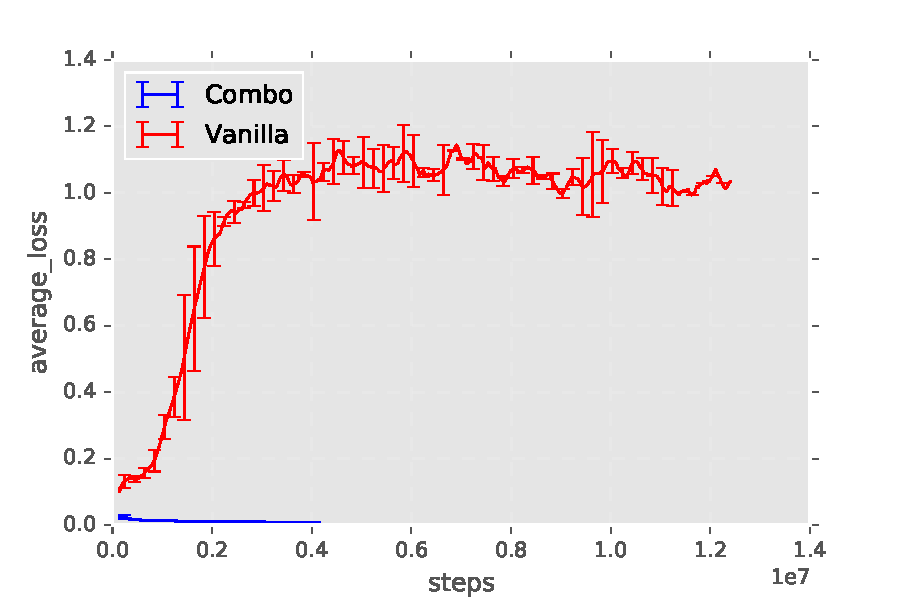
\includegraphics[width=0.5\textwidth]{../results/Krull/Comparisons/Combo/Combo-baseline-average_loss.pdf}
\end{figure}


\begin{figure}
    \centering
    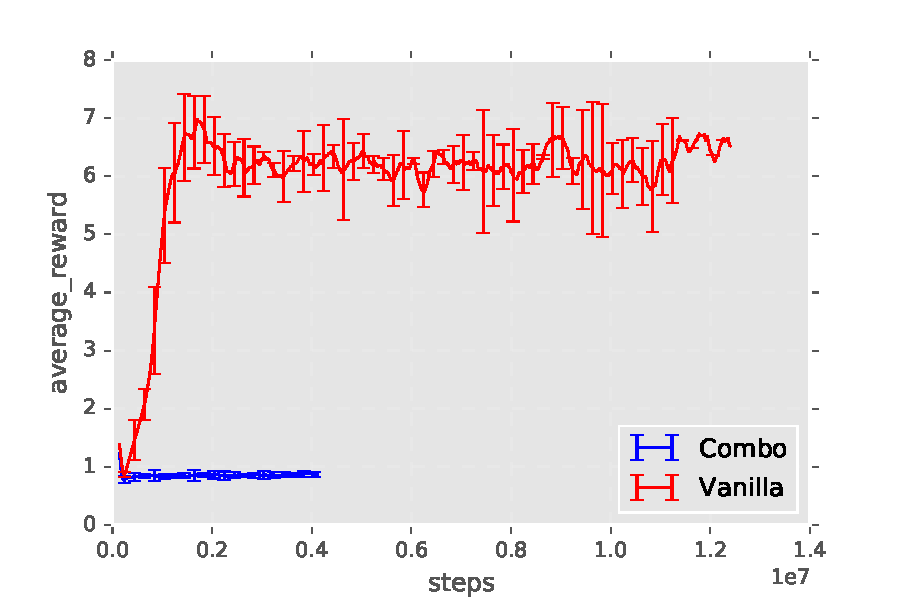
\includegraphics[width=0.5\textwidth]{../results/Krull/Comparisons/Combo/Combo-baseline-average_reward.pdf}
\end{figure}

\begin{figure}
    \centering
    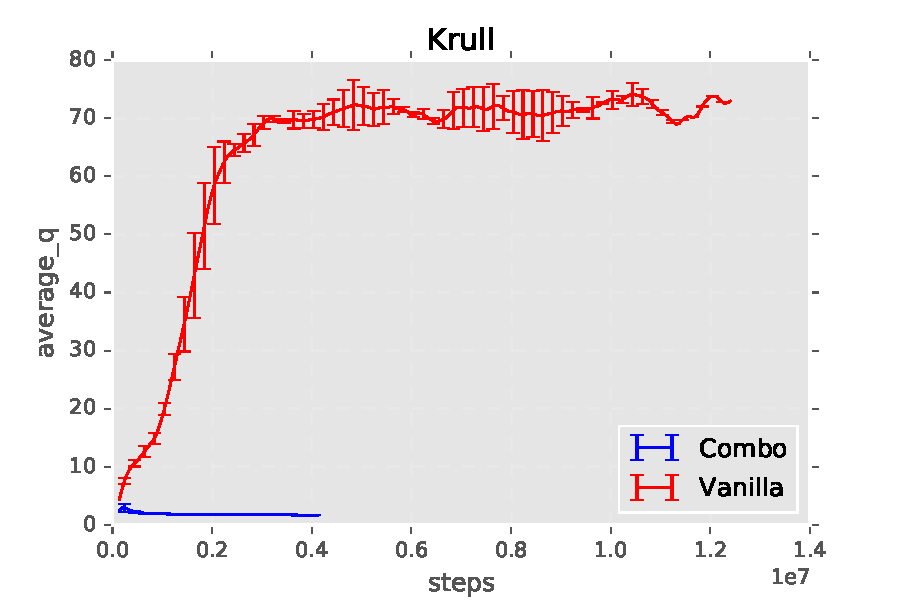
\includegraphics[width=0.5\textwidth]{../results/Krull/Comparisons/Combo/Combo-baseline-average_q.pdf}
\end{figure}

\begin{figure}
    \centering
    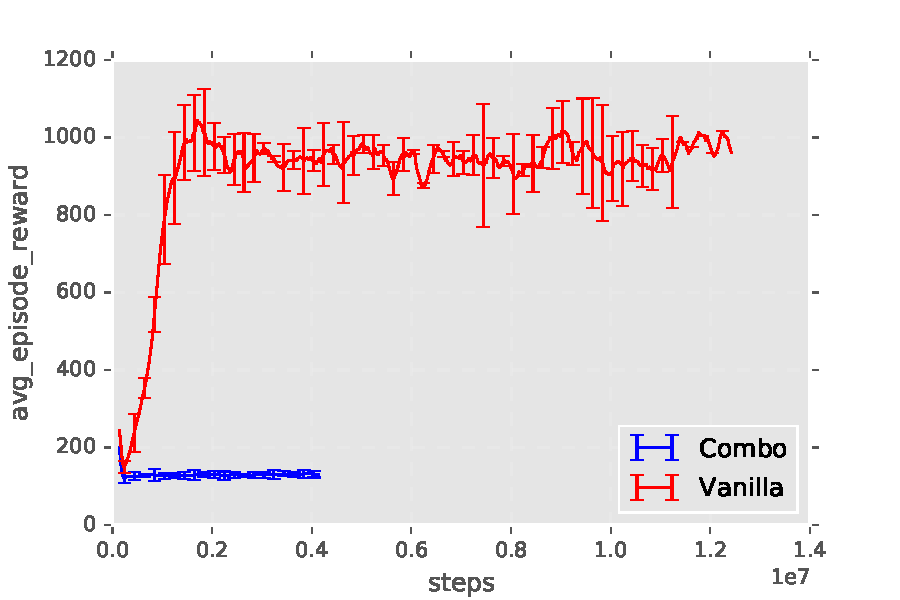
\includegraphics[width=0.5\textwidth]{../results/Krull/Comparisons/Combo/Combo-baseline-avg_episode_reward.pdf}
\end{figure}

\begin{figure}
    \centering
    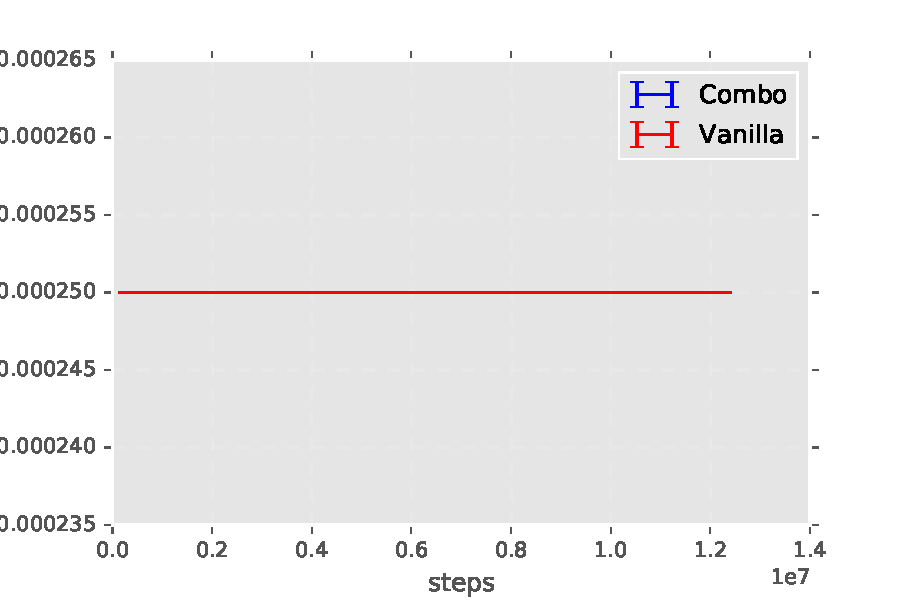
\includegraphics[width=0.5\textwidth]{../results/Krull/Comparisons/Combo/Combo-baseline-learning_rate.pdf}
\end{figure}


\begin{figure}
    \centering
    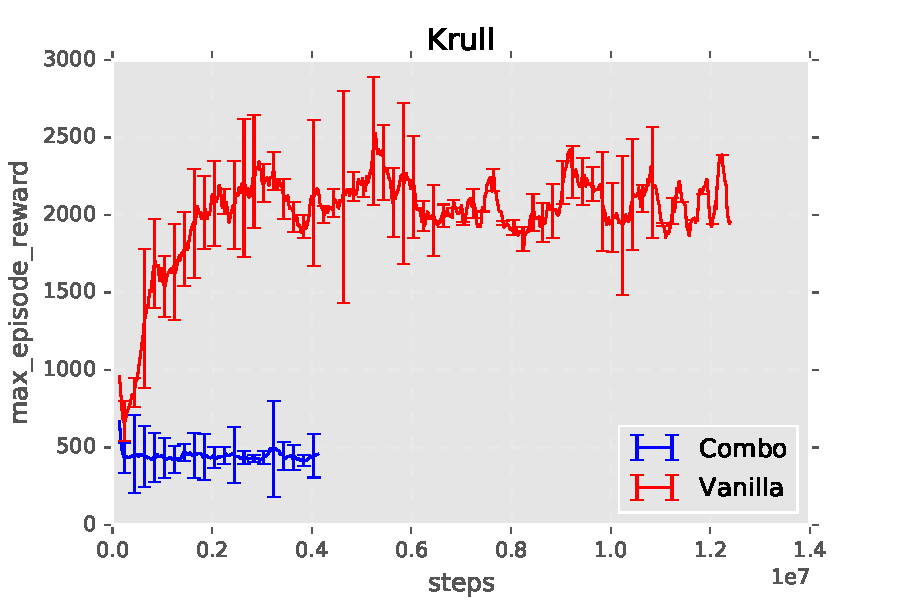
\includegraphics[width=0.5\textwidth]{../results/Krull/Comparisons/Combo/Combo-baseline-max_episode_reward.pdf}
\end{figure}


\begin{figure}
    \centering
    \includegraphics[width=0.5\textwidth]{../results/Krull/Comparisons/Combo/Combo-baseline-min_episode_reward.pdf}
\end{figure}
\FloatBarrier

\subsection{Boxing}\label{Appendix boxing prior}

\begin{figure}
    \centering
    \includegraphics[width=0.5\textwidth]{../results/Boxing/Comparisons/Combo/Combo-baseline-average_episode_num_of_games.pdf}
\end{figure}


\begin{figure}
    \centering
    \includegraphics[width=0.5\textwidth]{../results/Boxing/Comparisons/Combo/Combo-baseline-average_loss.pdf}
\end{figure}


\begin{figure}
    \centering
    \includegraphics[width=0.5\textwidth]{../results/Boxing/Comparisons/Combo/Combo-baseline-average_reward.pdf}
\end{figure}

\begin{figure}
    \centering
    \includegraphics[width=0.5\textwidth]{../results/Boxing/Comparisons/Combo/Combo-baseline-average_q.pdf}
\end{figure}

\begin{figure}
    \centering
    \includegraphics[width=0.5\textwidth]{../results/Boxing/Comparisons/Combo/Combo-baseline-avg_episode_reward.pdf}
\end{figure}

\begin{figure}
    \centering
    \includegraphics[width=0.5\textwidth]{../results/Boxing/Comparisons/Combo/Combo-baseline-learning_rate.pdf}
\end{figure}


\begin{figure}
    \centering
    \includegraphics[width=0.5\textwidth]{../results/Boxing/Comparisons/Combo/Combo-baseline-max_episode_reward.pdf}
\end{figure}


\begin{figure}
    \centering
    \includegraphics[width=0.5\textwidth]{../results/Boxing/Comparisons/Combo/Combo-baseline-min_episode_reward.pdf}
\end{figure}

\FloatBarrier



\end{document}